\input{header.tex}
\begin{document}
\selectlanguage{english}
%----------------------------------------------------------------%
%----------------------Titelseite--------------------------------%
%----------------------------------------------------------------%
% !TEX root = main.tex
\title{\textcolor{red}{Erdfeld-NMR Remote}}
\subtitle{Physikalisches Fortgeschrittenenpraktikum an der Universität Konstanz}
\author{Autoren: Philipp Gebauer, Simon Keegan und Marc Neumann \\ \large{Tutor: Narinder Narinder}}
\date{Versuch durchgeführt am 9. Juli 2020 und \textcolor{red}{???}}
\maketitle
\begin{abstract}
    \begin{center}
        \Large{\textsf{\textbf{Abstract}}}
    \end{center}
    \vspace{0.75 cm}
    \begin{singlespace}
    \noindent TEXT
    \vspace{0.75 cm}
     
    \noindent Beide Autoren haben zu jedem Abschnitt wesentliche Beiträge geleistet. Die Autoren bestätigen, dass sie die Ausarbeitung selbstständig verfasst haben und alle genutzten Quellen angegeben wurden.

\end{singlespace}
\end{abstract}

\thispagestyle{empty}
\newpage
%----------------------------------------------------------------%
%----------------------Inhaltsverzeichnis------------------------%
%----------------------------------------------------------------%
\tableofcontents
\thispagestyle{empty}
\newpage
\setcounter{page}{1} 
%---------------------------------------------------------------%
%----------------------Einleitung--------------------------------%
%----------------------------------------------------------------%
\input{Kapitel/1-einleitung}
%----------------------------------------------------------------%
%----------------------Grundlagen--------------------------------%
%----------------------------------------------------------------%

%----------------------------------------------------------------%
%-----------------------Aufbau und Durchführung------------------%
%---------------------------------------------------------------%
% !TEX root = main.tex
\section{Setup}
\label{sec:Aufbau}
This chapter is about the setup of this experiment. To understand which part of the experiment has what use, it is necessary to have a look at the components of the setup.\newline
Figure \ref{fig:Aufbau} shows the different coils which are necessary for the EFNMR measurement. The innerst coil B$_1$ is the excite and collect coil which is described in the previous chapter. The outer coil is to prepolarize the sample. This is necessary to obtain a stronger signal. By applying a strong magnetic field, all spins align in the direction of the prepolarising pulse and provides a bulk polarised nuclear magnetisation across the sample. The middle coil is the gradient coil. This coil erases the inhomogeneous magnetic field which always occurs for different uncertainty reasons. This coil is also used for the 2D imaging of the probe by adjusting the components of the magnetic field. The z-axis of the whole setup of the coils has to be aligned parallel to the earths magnetic field. Therefore a compass can be used to adjust the position. Via the computer program \textit{Prospa} and the spectrometer, the currents of the coil can be adjusted and the induced signals can be measured.
\begin{figure}[H]
    \centering
    \includegraphics[width= \textwidth]{Abbildungen/Aufbau.png}   
    \caption[Setup of the \textit{Terranova-MRI EFNMR}. \cite{Bild}]{Setup of the \textit{Terranova-MRI EFNMR}. On the left handside the coils B$_1$ (excite and collect coil), gradient coil (homogeneous magnetic field and 2D scanning coil) and the prepolarising coil B$_p$ are seen. The right hand side shows the water sample which has been used and the spectrometer which adjusts the necessary signals to the coils. \cite{Bild}}
    \label{fig:Aufbau}
\end{figure}

% !!!!!!!!
% !!!!!!!!!!
% !!!!!!!!!
% %Einstellen von größe des Bidles mit epslatex:  \resizebox{0.5\textwidth}{!}{\input{plots/Belichtungszeit.tex}}
% !!!!!!!!!!
% !!!!!!!!!!!
% !!!!!!!!!
\newpage
%----------------------------------------------------------------%
%----------------------Auswertung--------------------------------%
%----------------------------------------------------------------%
% !TEX root = main.tex
\section{Part I -- Basics}
\label{sec:PartI}
This part of the report discusses all the measurments made on the first day of the experiment and their analysis.
The focus is therefore on the basics of this whole experiment. Those include a noise measurment, an basic analysis of the used coils, elementary characterizations of a water sample and tuning the setup on this, an analysis of the  longitudinal and transversal relaxation times $T_1$ and $T_2$ respectively as well as the principle of \textsc{Hahn} echos and different possible applications of it.
%----------------------------------------------------------------%
%----------------------Teil I------------------------------------%
%----------------------------------------------------------------%
% !TEX root = main.tex
\section{Noisemeasurement}
\label{sec:Noisemeasurement}
The first step in the EFNMR Remote experiment is to measure the external noise. The external noise depends on the location where the setup is placed, the orientation of the probe and by surrounding metal objects e.g. a metal desk. To detect this external noise, a measurement without an NMR signal is provided. The time domain noise signal is shwon in figure \ref{fig: noise}. It is clearly visible that the noise is centered around \SI{0}{\mu \volt}. To gain knowledge about the noise level, the computer calculates the root-mean-square (RMS). This means that it calculates the square of each data point, than sum up all the squared values, calculates the average and than applies a square root. With this method the noise level can be calculated. In this case it is \SI{7.5}{\mu \volt}. This is an acceptable noise value, because any value below \SI{10}{\mu \volt} is good enough to provide good NMR data.

\begin{figure}[H]
    \centering
    \input{plots/noise.tex}
    \caption[Noise signal taken by the B$_1$ coil.]{Noise signal taken by the B$_1$ coil. The noise value of this noise is \SI{7.5}{\mu \volt}.}
    \label{fig: noise}
\end{figure}

Figure \ref{fig: MonitorNoise138} shows the frequency domain noise. This means that the time domain is fourier transformed into the frequency domain. This method is one of the basic principles we use in this experiment to make research about the properties of the measured signals. The frequency domain noise shows very specific sharp peaks every \SI{50}{\hertz}. To be more specific the peaks in the middle of every hundred \si{\hertz} steps are way higher than those at \SI{1400}{\hertz}, \SI{1500}{\hertz} and so on. This results of the frequency in the power grid which is \SI{50}{\hertz} in Germany and can also be affiliated to the electrical noise of a surrounding fluorescent light or the CRT computer monitor. Unfortunately the remote camera program of the computer did not work and therefore it is not clear if there was a fluorescent light in the room. Even though the noise peaks in the frequency domain figure indicates that there could be a fluorescent light source in the room.
Despite all sharp peaks there is also a slight increase of the amplitude around $\SI{185 \pm 10}{\cdot 10^1 \frac{\mu \volt}{\hertz}}$ visible. This is explicable by the resonance frequency of the instrument and its sensitvity around the lamorfrequency (\SI{1841.4}{\hertz} for water in Germany in July 2020). All our following measurements will be done nearby the lamorfrequency. That is why the instrument sensitvity is sharpend around this value.

\begin{figure}[H]
    \centering
    \input{plots/MonitorNoise138.tex}
    \caption[Fourier transformed noise signal of the previous figure \ref{fig: noise}.]{Fourier transformed noise signal of the previous figure \ref{fig: noise}. Strong peaks every \SI{50}{\hertz} correspond to the frequency of the power grid in Germany and to electrical noise of a surrounding fluorescent light or the CRT computer monitor. The slight increase of the amplitude around $\SI{185 \pm 10}{\cdot 10^1 \frac{\mu \volt}{\hertz}}$ is explicable by the resonance frequency of instrument and its sensitvity around the lamorfrequency (\SI{1841.4}{\hertz} for water in Germany in July 2020).}
    \label{fig: MonitorNoise138}
\end{figure}


% !TEX root = main.tex
\subsection{Coil Analysis}
\label{sec:CoilAnalyssis}
Now knowing that we have an acceptable noise value of less than \SI{10}{\mu \volt}, we can analyse the coil.
In order to do so we explain the general approach of NMR signals first.
To measure a NMR signal a pulse and collect measurement has to be done.
Therefore the B$_1$ coil (transmit and collect coil) has to apply a pulse.
This pulse changes the spins direction out of its thermal equilibrium (along z-axes, due to the earths magnetic field B$_e$) into a direction with a component in the transversal plain.
Therefore the B$_1$ coil collects a signal because it is aligned orthogonal to B$_e$.
The transmit and collect procedure is based on \textsc{Faraday}'s law of induction.
Figure \ref{fig: PulsandcollectValesignal} exemplary shows such a pulse and collect signal by the B$_1$ coil.
Every following measurement in this report is based on the procedure of pulse and collect.

\begin{figure}[H]
    \centering
    \input{plots/PulsandcollectValesignal.tex}
    \caption[Example signal for a pulse and collect signal made by the B$_1$ coil.]{Example signal for a pulse and collect signal made by the B$_1$ coil.
    The example signal is taken from a FID signal.}
    \label{fig: PulsandcollectValesignal}
\end{figure}

Due to the fact that the B$_1$ coil is a tuned LCR circuit a resonance frequency exists, which can be calculated by the following formula:
\begin{align}
    \omega_{calc} = \frac{1}{\sqrt{L \cdot C}} \ .
    \label{eq: larmorcalc}
\end{align}
In order to analyse the B$_1$ coil the resonance frequency, depending on the capacity, is measured.
Therefore the B$_1$ coil transmits a signal.
Due to this signal the response of the coil can be measured.
This signal is then fourier transformed and the resonance frequency can be deduced from the frequency domain (maximum in the frequency domain).
This procedure is repeated automatically by the computer programm \textit{Prospa} for different capacities.
By changing the capacity we can examine the best capacity in dependence of the larmor frequency.
Figure \ref{fig: Coilanalyse} shows the measured and theoretically calculated resonance frequency (equation \eqref{eq: larmorcalc}; $L = \SI{0.417}{\henry}$) in dependence of the capacity.
The horizontal line represents the larmor frequency of \SI{1841.4}{\hertz} for hydrogen in Germany in July 2020.
To gain this value the vertical component of the earths magnetic field (\SI{43248.8}{\nano \tesla} \cite{magnetfeld}) is multiplied by the gyromagnetic ratio $\SI{42.577}{\frac{\mega \hertz}{\tesla}}$ \cite{magnetfeld}.
The vertical line represents the correct capacity we should use for our measurement, due to the resonance frequency of the larmor frequency.
In this case the correct capacity is \SI{13.8}{\nano \farad}.
Corresponding to the calculated resonance frequency the correct capacity would be \SI{17.9}{\nano \farad}.
It is not deniable that the measured curve is not parallel to the measured resonance frequency.
This probably has its cause in the not fixed inductance $L$.
Due to heating of the coil $L$ might change a little by increasing capacity and thus the calculated curve does not fit to the measured one.
Another reason for the different calculated curve is that we used real coils and those have parasite resistances and also built-in capacities.
This built-in capacity is not taken into account in the formula \eqref{eq: larmorcalc} and therefore the calculated curve might be not correct.
Since the calculated curve does not fit to the measured one, the calculated value for the capacity is not taken into account.

\begin{figure}[H]
    \centering
    \input{plots/Coilanalyse.tex}
    \caption[This figure shows the measured and calculated resonance frequencies for different capacities.]{This figure shows the measured and calculated resonance frequencies for different capacities.
    The marked cross represents the larmor frequency of \SI{1841.4}{\hertz} for hydrogen in Germany in July 2020.}
    \label{fig: Coilanalyse}
\end{figure}
\newpage
% !TEX root = main.tex
\section{Optimization and Characterisation of FID in water sample}
\label{sec:OptimizationandCharacterisationofFIDinwatersample}

One of the main goals of this experiment is to measure a good FID of the water sample. In order to do so we first have to optimize our FID signal of the water probe.\newline
At first the inhomogeneity of the magnetic field has to be cancelled. The process to make the magnetic field more homogeneous is to \textit{autoshim} the components of the gradient coil. The computer programm does this automatically. So it deshims the system step by step and checks if the output maximizes or minimizes. By checking many different combinations it finds the best shimming values for the gradient coil. In our case they are:
\begin{align*}
    x &= \SI{10.11}{\milli \ampere}\\
    y &= \SI{20.88}{\milli \ampere}\\
    z &= \SI{-20.07}{\milli \ampere} \ .
    \label{eq: shimmingvalues}
\end{align*}
That means with those shimming values the magnetic field in the setup is homogeneous.
\\
The second optimization step is to change the B$_1$ pulse duration. The longer the pulse duration is, the bigger is the angle of the flipping spins and thus the signal will get stronger (only for flipping angles till \SI{90}{\degree}). The best signal is obtained for an flipping angle of \SI{90}{\degree}, because with this angle the spins only have a component in the transversal plane and therefore the signal is maximized. If the pulse duration is too long, than the flipping angle is bigger than \SI{90}{\degree} and the spins get a horizontal component again and the signal will decrease again. When a flipping angle of \SI{180}{\degree} is reached the signal will be at its minimum. Afterwards the signal will raise again, because of the increasing horizontal component. Figure \ref{fig:B1dauer} shows this issue. The maxmimum at a pulse duration of \SI{1.35}{\milli \second} is clearly visible. This means that after apllying a B$_1$ pulse with a duration of \SI{1.35}{\milli \second} the spins are in the transversal plane and therefore the best signal is obtained.
\begin{figure}[H]
    \centering
    \input{plots/B1dauer.tex}
    \caption[This figure shows which impact the B$_1$ pulse duration has to the ampitude of the FID.]{This figure shows which impact the B$_1$ pulse duration has to the ampitude of the FID. It is clearly visible that the duration has a maximum at \SI{1.35}{\milli \second} which is the duration for a \SI{90}{\degree} pulse.}
    \label{fig:B1dauer}
\end{figure}
Figure \ref{fig:pulsedurationbeispiel} exemplarily shows the correlation of the B$_1$ pulse duration and the signal which the coil detects. It is clearly visible that the amplitude is better for the pulse duration of \SI{1.35}{\milli \second} than for the pulse duration of \SI{0.27}{\milli \second}. The signal that was taken for the pulse duration of \SI{0.27}{\milli \second} is at the minimum of the figure \ref{fig:B1dauer} and therefore it is correct that the amplitude of the spectrum with the pulse duration of \SI{1.35}{\milli \second} is higher.
\begin{figure}[H]
    \centering
    \input{plots/138_puls_and_collect_number_of_delay25ms_Pulseduration0_27ms.tex}
    \caption[Example spectrum for two different B$_1$ pulse durations.]{Example spectrum for two different B$_1$ pulse durations. The peak which is higher corresponds to the \SI{1.35}{\milli \second} duration pulse and represents the \SI{90}{\degree} pulse. This peak is high, because at this duration most of the spins are in the transversal plane and therfore the amplitude is maximal.}
    \label{fig:pulsedurationbeispiel}
\end{figure}
Now that the B$_1$ pulse duration is also optimized, we can have a closer look at the capacity of the LCR circuit of the B$_1$ coil again. First it is necessary to know that the B$_1$ pulse is applied by a \textit{rectangular} function and the fourie transformation of a \textit{rectangular} function is a \textit{sinc} function. Therefore the fourier ransformed spectrum of the B$_1$ pulse signal is a \textit{sinc} function. When we measure the signal shortly (acquisition delay: \SI{2}{\milli \second}) after the \SI{90}{\degree} pulse, there shoud be a \textit{sinc} function visible and indeed this is what we obtained (figure \ref{fig:Pulsandcollect}). In figure \ref{fig:Pulsandcollect} there is also a really sharp peak visible. This is referd to the hydrogen signal. The hydrogen signal is independed of the applied capacity, but the $B_1$ pulse is, because the capacity changes the properties of the LCR-circuit of the B$_1$ coil. The best capacity is adjusted when the hydrogen signal is in the middle of the \textit{sinc} function, because then the LC- circuit is tuned to the lamor frequency of the hydrogen signal. This is also visible by the amplitude of the spectrum in figure \ref{fig:Pulsandcollect}. The amplitude of the spectrum which was observed for a capacity of \SI{13.8}{\nano \farad} is higher than for the amplitude of the spectrum which was observed for a capacity of \SI{14.2}{\nano \farad}. As already explained before in the chapter \ref{sec:CoilAnalyssis} the capacity of \SI{13.8}{\nano \farad} is indeed the best capacity in order to observe a maximized spectrum.
\begin{figure}[H]
    \centering
    \input{plots/Pulsandcollect138.tex}
    \caption[This figure shows the impact of the capacity in the LCR circuit of the B$_1$ coil.]{This figure shows the impact of the capacity in the LCR circuit of the B$_1$ coil. The \textit{sinc} function comes from the fourier transformed B$_1$ pulse, which is rectangular. The peak at \SI{1837.27 \pm 0.05}{\hertz} is the peak from the hydrogen signal.}
    \label{fig:Pulsandcollect}
\end{figure}
Now that the FID signal is optimized best we can start to characterize it. Therefore we measure a FID with a acquisition delay of \SI{25}{\milli \second}, because after this delay there are no effects from the rectangular applied B$_1$ pulse anymore (no \textit{sinc} function in the spectrum). The figure \ref{fig:Pulsandcollect138_delay_25_gauss} shows the observed spectrum and two different fit possibilities.\newline
One option to fit a peak in a spectrum is by applying a \textit{voigt}-profile ($V(x;\sigma , \gamma)$). This function is a convolution of the \textit{Cauchy-Lorentz}- and \textit{Gaussian}-distribution and is described by following formula:
\begin{align}
    V(x;\sigma , \gamma) &= ( G \star L)(x) = \int G(\tau) L(x-\tau) d\tau \\
    G(x;\sigma) &= \frac{exp\left(\frac{-x^2}{2\sigma^2}\right)}{\sigma \sqrt{2 \pi}} \\
    L(x;\gamma)  &= \frac{\gamma}{\pi \left( x^2+\gamma^2\right)} \ .
    \label{eq: voigt} 
\end{align}
$\sigma$ represents the standard deviation, $\gamma$ is half of the peak width at half height from the \textit{Lorentz}-distribution and $x$ is the shift from the line center. In figure \ref{fig:Pulsandcollect138_delay_25_gauss} the \textit{voigt}-profile (green) is fitted to the measured spectrum (red). The problem about this fit is that is not as sharp as the measured data. This might be, due to the fact that the measured spectrum does not have many data points especially around the maximum. Therefore the peak is really sharp and a correct fit with the \textit{voigt}-profile is rather difficult. Therefore a second fit function has been apllied. This time only the \textit{Gaussian}-distribution. This fit function is better to calculate the width of the peak, due to the fact that it is easier to fit it to this narrow peak. The full width of the peak at have maximum (FWHM) is calculated by the applied \textit{Gaussian}-fit and is \SI{1.177 \pm 0.042}{\hertz}. \newline
The amplitude of the peak is \SI{73.85}{\mu \volt} according to the \textit{Gaussian}-fit and is in comparison to the amplitude of the noise measurement (magnitude \SI{1}{}) in figure \ref{fig: MonitorNoise138} high. The signal to noise ratio of this point is \SI{47.57}{}. To calculate this value the amplitude at \SI{1837.27}{\hertz} (center of the peak) in figure \ref{fig:Pulsandcollect138_delay_25_gauss} is devided by the value of the amplitude at the same frequency in figure \ref{fig: MonitorNoise138}. That value clearly shows that the peak must come from the hydrogen signal and is barely disturbed by any noise.\newline
The width of the measured hydrogen peak at half hight (FWHM) is \SI{1.180 \pm 0.040} and therefore really sharp. An even better value can only be achieved by tuning the setup even more. To show the physical properties this value is though of a really good size.\newline
The disadvantage of the \textit{Gaussian}-fit is that area under the curve does not equal the measured one, especially around \SI{1836}{\hertz} and \SI{1839}{\hertz}. Therefore the discussion about the integral under the measured curve will just be qualitative and will be done in the chapter \ref{sec:Hahnecho}.\newline
It is also possible to take a measurement of the imaginary signal of the peak in figure \ref{fig:Pulsandcollect138_delay_25_gauss}. Unfortunately we did not safe this data. Therefore we explain what we should see and what it means. The imaginary component discribes the dispersion spectrum. The spectrum then has to look like kind of a hyperbolic function with the pole exactly at \SI{1837.27}{\hertz} (center of the peak). Since it is no real hyperbolic function there exist values at the pole. Those values are aligned in a vertical line.
\begin{figure}[H]
    \centering
    % GNUPLOT: LaTeX picture with Postscript
\begingroup
  % Encoding inside the plot.  In the header of your document, this encoding
  % should to defined, e.g., by using
  % \usepackage[cp1252,<other encodings>]{inputenc}
  \inputencoding{cp1252}%
  \makeatletter
  \providecommand\color[2][]{%
    \GenericError{(gnuplot) \space\space\space\@spaces}{%
      Package color not loaded in conjunction with
      terminal option `colourtext'%
    }{See the gnuplot documentation for explanation.%
    }{Either use 'blacktext' in gnuplot or load the package
      color.sty in LaTeX.}%
    \renewcommand\color[2][]{}%
  }%
  \providecommand\includegraphics[2][]{%
    \GenericError{(gnuplot) \space\space\space\@spaces}{%
      Package graphicx or graphics not loaded%
    }{See the gnuplot documentation for explanation.%
    }{The gnuplot epslatex terminal needs graphicx.sty or graphics.sty.}%
    \renewcommand\includegraphics[2][]{}%
  }%
  \providecommand\rotatebox[2]{#2}%
  \@ifundefined{ifGPcolor}{%
    \newif\ifGPcolor
    \GPcolorfalse
  }{}%
  \@ifundefined{ifGPblacktext}{%
    \newif\ifGPblacktext
    \GPblacktexttrue
  }{}%
  % define a \g@addto@macro without @ in the name:
  \let\gplgaddtomacro\g@addto@macro
  % define empty templates for all commands taking text:
  \gdef\gplbacktext{}%
  \gdef\gplfronttext{}%
  \makeatother
  \ifGPblacktext
    % no textcolor at all
    \def\colorrgb#1{}%
    \def\colorgray#1{}%
  \else
    % gray or color?
    \ifGPcolor
      \def\colorrgb#1{\color[rgb]{#1}}%
      \def\colorgray#1{\color[gray]{#1}}%
      \expandafter\def\csname LTw\endcsname{\color{white}}%
      \expandafter\def\csname LTb\endcsname{\color{black}}%
      \expandafter\def\csname LTa\endcsname{\color{black}}%
      \expandafter\def\csname LT0\endcsname{\color[rgb]{1,0,0}}%
      \expandafter\def\csname LT1\endcsname{\color[rgb]{0,1,0}}%
      \expandafter\def\csname LT2\endcsname{\color[rgb]{0,0,1}}%
      \expandafter\def\csname LT3\endcsname{\color[rgb]{1,0,1}}%
      \expandafter\def\csname LT4\endcsname{\color[rgb]{0,1,1}}%
      \expandafter\def\csname LT5\endcsname{\color[rgb]{1,1,0}}%
      \expandafter\def\csname LT6\endcsname{\color[rgb]{0,0,0}}%
      \expandafter\def\csname LT7\endcsname{\color[rgb]{1,0.3,0}}%
      \expandafter\def\csname LT8\endcsname{\color[rgb]{0.5,0.5,0.5}}%
    \else
      % gray
      \def\colorrgb#1{\color{black}}%
      \def\colorgray#1{\color[gray]{#1}}%
      \expandafter\def\csname LTw\endcsname{\color{white}}%
      \expandafter\def\csname LTb\endcsname{\color{black}}%
      \expandafter\def\csname LTa\endcsname{\color{black}}%
      \expandafter\def\csname LT0\endcsname{\color{black}}%
      \expandafter\def\csname LT1\endcsname{\color{black}}%
      \expandafter\def\csname LT2\endcsname{\color{black}}%
      \expandafter\def\csname LT3\endcsname{\color{black}}%
      \expandafter\def\csname LT4\endcsname{\color{black}}%
      \expandafter\def\csname LT5\endcsname{\color{black}}%
      \expandafter\def\csname LT6\endcsname{\color{black}}%
      \expandafter\def\csname LT7\endcsname{\color{black}}%
      \expandafter\def\csname LT8\endcsname{\color{black}}%
    \fi
  \fi
    \setlength{\unitlength}{0.0500bp}%
    \ifx\gptboxheight\undefined%
      \newlength{\gptboxheight}%
      \newlength{\gptboxwidth}%
      \newsavebox{\gptboxtext}%
    \fi%
    \setlength{\fboxrule}{0.5pt}%
    \setlength{\fboxsep}{1pt}%
\begin{picture}(7200.00,5040.00)%
    \gplgaddtomacro\gplbacktext{%
      \csname LTb\endcsname%%
      \put(682,704){\makebox(0,0)[r]{\strut{}$0$}}%
      \put(682,1161){\makebox(0,0)[r]{\strut{}$10$}}%
      \put(682,1618){\makebox(0,0)[r]{\strut{}$20$}}%
      \put(682,2076){\makebox(0,0)[r]{\strut{}$30$}}%
      \put(682,2533){\makebox(0,0)[r]{\strut{}$40$}}%
      \put(682,2990){\makebox(0,0)[r]{\strut{}$50$}}%
      \put(682,3447){\makebox(0,0)[r]{\strut{}$60$}}%
      \put(682,3905){\makebox(0,0)[r]{\strut{}$70$}}%
      \put(682,4362){\makebox(0,0)[r]{\strut{}$80$}}%
      \put(682,4819){\makebox(0,0)[r]{\strut{}$90$}}%
      \put(814,484){\makebox(0,0){\strut{}$1830$}}%
      \put(1613,484){\makebox(0,0){\strut{}$1832$}}%
      \put(2411,484){\makebox(0,0){\strut{}$1834$}}%
      \put(3210,484){\makebox(0,0){\strut{}$1836$}}%
      \put(4008,484){\makebox(0,0){\strut{}$1838$}}%
      \put(4807,484){\makebox(0,0){\strut{}$1840$}}%
      \put(5605,484){\makebox(0,0){\strut{}$1842$}}%
      \put(6404,484){\makebox(0,0){\strut{}$1844$}}%
      \put(4208,2304){\makebox(0,0)[l]{\strut{}FWHM $= \SI{1.177 \pm 0.042}{\hertz}$}}%
      \put(4208,2762){\makebox(0,0)[l]{\strut{}$\sigma =  \SI{0.500 \pm 0.018}{\hertz}$}}%
    }%
    \gplgaddtomacro\gplfronttext{%
      \csname LTb\endcsname%%
      \put(209,2761){\rotatebox{-270}{\makebox(0,0){\strut{}Amplitude in $\si{\mu \volt}$}}}%
      \put(3808,154){\makebox(0,0){\strut{}Frequency in $\si{\hertz}$}}%
      \csname LTb\endcsname%%
      \put(5816,4646){\makebox(0,0)[r]{\strut{}magnitude spectrum}}%
      \csname LTb\endcsname%%
      \put(5816,4426){\makebox(0,0)[r]{\strut{}voigt-profile}}%
      \csname LTb\endcsname%%
      \put(5816,4206){\makebox(0,0)[r]{\strut{}\textsc{Gauss}-Fit}}%
    }%
    \gplbacktext
    \put(0,0){\includegraphics{plots/Pulsandcollect138_delay_25_gauss}}%
    \gplfronttext
  \end{picture}%
\endgroup

    \caption[This figure shows the measured hydrogen signal after an acquisition delay of \SI{25}{\milli \second} and two possible ways to fit the peak.]{This figure shows the measured hydrogen signal after an acquisition delay of \SI{25}{\milli \second} and two possible ways to fit the peak. Due to a very short frequency range the peak looks very wide. Indeed it is actually very sharp. To fit the peak a \textit{voigt}-profile and \textit{Gaussian}-fit is used.}
    \label{fig:Pulsandcollect138_delay_25_gauss}
\end{figure}
% !TEX root = main.tex
\section{Longitudinal relaxation measurements T1}
\label{sec:LongitudinalrelaxationmeasurementsT1}
There exist two possibilities to measure the longitudinal spin lattice relaxation.
First we want to have a closer look at the measurement via $\tau_p$ (polarizing pulse duration).
Therefore the computer program \textit{Prospa} applies a polarizing pulse orthogonal to the earths magnetic field.
Due to this polarizing pulse the spins align in the transversal plain and form a bulk magnetization.
By time the magnetization becomes stronger because of this the signal becomes stronger.
This relation is visualized in the figure \ref{fig:BildT1}.

\begin{figure}[H]
    \centering
    \includegraphics[width= \textwidth]{Abbildungen/BildT1.png}   
    \caption[Sketch to show how T$_1$ can be measured. \cite{Bild}]{Sketch to show how T$_1$ can be measured.
    One way is by changing the polarizing pulse duration $\tau_p$ and the other way is by varying the time between the polarizing pulse and the \SI{90}{\degree} pulse. \cite{Bild}}
    \label{fig:BildT1}
\end{figure}

Due to the increasing magnetization it is possible to calculate the T$_{1,p}$ relaxation.
In order to do so the magnetization time is increased step by step from \SI{500}{\milli \second} to \SI{4500}{\milli \second} with an increment of \SI{500}{\milli \second} and in each configuration the signals maximum is obtained from the fourier transformed spectrum.
Figure \ref{fig:T1Polarisationsfeldfeld} shows the attenuation of the signals normalized to the maximum peak E$_0$.
The underlying idea is that by applying a fit function as following:
\begin{align}
    S(x)=S_0 \cdot \left[1-\exp\left(\frac{-x}{T_{1,p}}\right)\right] \ ,
    \label{eq: fitBp}
\end{align}
it is possible to calculate the relaxation time T$_{1,p}$.
The exponential decay is a result of the loss of phase coherence between the spins and will be used for every measurement of spin relaxation.
In this case T$_{1,p}$ is found to count as \SI{2912.8800 \pm 0.0048}{\milli \second}.

\begin{figure}[H]
    \centering
    \input{plots/T1Polarisationsfeldfeld.tex}
    \caption[T$_{1,p}$ measurement by varying $\tau_p$ and observing how the attenuation $\frac{\text{E}}{\text{E}_0}$ evolves.]{T$_{1,p}$ measurement by varying $\tau_p$ and observing how the attenuation $\frac{\text{E}}{\text{E}_0}$ evolves.
    The provided exponential fit results in a value for T$_{1,p}$ of \SI{2912.8800 \pm 0.0048}{\milli \second}.}
    \label{fig:T1Polarisationsfeldfeld}
\end{figure}

The second option is to calculate the spin lattice relaxation via the earths magnetic field B$_e$.
In this case the index will be chosen as "$e$" for the spin lattice relaxation.
The procedure in this case is to change the time $t$ (pre-90 minimum delay) between the polarizing pulse ends and the \SI{90}{\degree} pulse begins.
This relation is also visualized in figure \ref{fig:BildT1}.
The pre-90 minimum delay is chosen as \SI{0}{\milli \second} and the pre-90 delay step size as \SI{500}{\milli \second}.
For every configuration the signal maximum is calculated again of the fourier transformed spectrum.
Figure \ref{fig:T1Erdmagnetfeld} shows the attenuation of the signals normalized to the maximum peak E$_0$.
This time the T$_{1,e}$ can be calculated by the following fit function:
\begin{align}
    S(x) = S_0 \cdot \exp\left(\frac{-x}{T_{1,e}}\right) \ .
    \label{eq: fitBe}
\end{align}
In our case T$_{1,e}$ is observed to be \SI{2753.0500 \pm 0.0012}{\milli \second}.\newline
In both ways the uncertainty of the T$_1$ values are quite small.
This is the result of really good aligned values to the fit function.
Nevertheless T$_{1,p}$ and T$_{1,e}$ are not consistent even though the uncertainty is considered.
This might be, due to the fact that those two measurements are based on two different methods and T$_{1,e}$ is dependent on the earths magnetic field.
Even though they are not consistent, the values for T$_{1,p}$ and T$_{1,e}$ have the same magnitude and also have the same magnitude according to a literature value of \SI{4000}{\milli \second} \cite{literaturT1}.
It is good to keep in mind that a comparison to literature values is just there to get the magnitude.
Since the surrounding magnetic field and the probe define the exact value.
\begin{figure}[H]
    \centering
    \input{plots/T1Erdmagnetfeld.tex}
    \caption[T$_{1,e}$ measurement by varying $t$ and observing how the attenuation $\frac{\text{E}}{\text{E}_0}$ evolves.]{T$_{1,e}$ measurement by varying $t$ and observing how the attenuation $\frac{\text{E}}{\text{E}_0}$ evolves.
    The provided exponential fit results in a value for T$_{1,e}$ of \SI{2753.0500 \pm 0.0012}{\milli \second}.}
    \label{fig:T1Erdmagnetfeld}
\end{figure}
% !TEX root = main.tex
\section{Hahn echo}
\label{sec:Hahnecho}
The other relaxation measurement is the T$_2$ measurement. In order to understand that, we first have to explain the \textit{Hahn} echo and the principle of multiple echo sequences.\newline
The principle of the \textit{Hahn} echo is that an \SI{90}{\degree} pulse is applied and after a certain time $\tau$ a \SI{180}{\degree} pulse. The reason behind this method is that after the \SI{90}{\degree} pulse the spins are oriented in the transversal plane and start to precise around the earths magnetic field vector (z-axis). Due to spin-spin interaction (inhomogeneous magnetic field accrues) the spins also interact with each other and therefore some spins have a higher larmor frequency and some have a lower one. If an \SI{180}{\degree} pulse is applied after a certain time the spins will flip in the transversal plane and the slow precessing spins will be before the fast precessing spins again and when the fast precessing  overtake the slow ones again the B$_1$ coil will detect a signal again. The reason why the B$_1$ coil does not detect something while the slow and fast precessing spins are at different position is that they erase each other. If the spin-spin interaction is too weak than it also helps to deshim the system along the x-direction. This also makes the homogeneous magnetic field inhomogeneous and thus the spins will get different larmor frequencies according to there position.\newline
Figure \ref{fig:Echobeispeilsignal} exemplarily shows the \textit{Hahn} echo for a shimming value of \SI{4.95}{\milli \ampere} along the x-axis (original value \SI{10.11}{\milli \ampere}). It is also possible to change the time between the \SI{90}{\degree} and \SI{180}{\degree} pulse. This would shift the peak to higher times in the timescale and due to loss effects, the amplitude will shrink a little bit.
\begin{figure}[H]
    \centering
    \input{plots/Echobeispeilsignal.tex}
    \caption[Example of a single \textit{Hahn} echo for an echo time of \SI{0}{\milli \second}.]{Example of a single \textit{Hahn} echo for an echo time of \SI{0}{\milli \second}. The maximum of the echo is clearly visible. Due to relaxation after the maximum the signal after about \SI{0.2}{\second} is noise.}
    \label{fig:Echobeispeilsignal}
\end{figure}
It is also possible to fourier transform the signal from figure \ref{fig:Echobeispeilsignal}. Figure \ref{fig:SpinEcho} shows this for two different shimming values. The amplitude of the spectrum with the shimming value of \SI{0}{\milli \ampere} along the x-axis is clearly smaller than the amplitude of the spectrum with shimming value of \SI{4.95}{\milli \ampere} along the x-axis. This effect comes from the more inhomogeneous magnetic field of the spectrum with the shimming value of \SI{0}{\milli \ampere} along the x-axis. A more inhomogeneous magnetic field also means that the spins have more different larmor frequencies and thus the total intensity will shrink. The area under the spectrum should be independent from the inhomogeneity, because in total the magnetisation has to be the same. Only the distribution is different. This effect is also really good visible in the figure \ref{fig:SpinEcho}. This time it is not possible to find a good fitting function. Therefore this discussion is more qualitativ as mentioned before in chapter \ref{sec:OptimizationandCharacterisationofFIDinwatersample}. The reason why there is no good fitting function is that there are a lot of random peaks in the spectrum and the more peaks there are the more difficult it is to find a good fitting function. Another thing which makes it rather hard is that the frequency steps are not very small and thus there are not many datapoints to make a good fit. This was also a problem in chapter \ref{sec:OptimizationandCharacterisationofFIDinwatersample} as mentioned before.
\begin{figure}[H]
    \centering
    % GNUPLOT: LaTeX picture with Postscript
\begingroup
  % Encoding inside the plot.  In the header of your document, this encoding
  % should to defined, e.g., by using
  % \usepackage[cp1252,<other encodings>]{inputenc}
  \inputencoding{cp1252}%
  \makeatletter
  \providecommand\color[2][]{%
    \GenericError{(gnuplot) \space\space\space\@spaces}{%
      Package color not loaded in conjunction with
      terminal option `colourtext'%
    }{See the gnuplot documentation for explanation.%
    }{Either use 'blacktext' in gnuplot or load the package
      color.sty in LaTeX.}%
    \renewcommand\color[2][]{}%
  }%
  \providecommand\includegraphics[2][]{%
    \GenericError{(gnuplot) \space\space\space\@spaces}{%
      Package graphicx or graphics not loaded%
    }{See the gnuplot documentation for explanation.%
    }{The gnuplot epslatex terminal needs graphicx.sty or graphics.sty.}%
    \renewcommand\includegraphics[2][]{}%
  }%
  \providecommand\rotatebox[2]{#2}%
  \@ifundefined{ifGPcolor}{%
    \newif\ifGPcolor
    \GPcolorfalse
  }{}%
  \@ifundefined{ifGPblacktext}{%
    \newif\ifGPblacktext
    \GPblacktexttrue
  }{}%
  % define a \g@addto@macro without @ in the name:
  \let\gplgaddtomacro\g@addto@macro
  % define empty templates for all commands taking text:
  \gdef\gplbacktext{}%
  \gdef\gplfronttext{}%
  \makeatother
  \ifGPblacktext
    % no textcolor at all
    \def\colorrgb#1{}%
    \def\colorgray#1{}%
  \else
    % gray or color?
    \ifGPcolor
      \def\colorrgb#1{\color[rgb]{#1}}%
      \def\colorgray#1{\color[gray]{#1}}%
      \expandafter\def\csname LTw\endcsname{\color{white}}%
      \expandafter\def\csname LTb\endcsname{\color{black}}%
      \expandafter\def\csname LTa\endcsname{\color{black}}%
      \expandafter\def\csname LT0\endcsname{\color[rgb]{1,0,0}}%
      \expandafter\def\csname LT1\endcsname{\color[rgb]{0,1,0}}%
      \expandafter\def\csname LT2\endcsname{\color[rgb]{0,0,1}}%
      \expandafter\def\csname LT3\endcsname{\color[rgb]{1,0,1}}%
      \expandafter\def\csname LT4\endcsname{\color[rgb]{0,1,1}}%
      \expandafter\def\csname LT5\endcsname{\color[rgb]{1,1,0}}%
      \expandafter\def\csname LT6\endcsname{\color[rgb]{0,0,0}}%
      \expandafter\def\csname LT7\endcsname{\color[rgb]{1,0.3,0}}%
      \expandafter\def\csname LT8\endcsname{\color[rgb]{0.5,0.5,0.5}}%
    \else
      % gray
      \def\colorrgb#1{\color{black}}%
      \def\colorgray#1{\color[gray]{#1}}%
      \expandafter\def\csname LTw\endcsname{\color{white}}%
      \expandafter\def\csname LTb\endcsname{\color{black}}%
      \expandafter\def\csname LTa\endcsname{\color{black}}%
      \expandafter\def\csname LT0\endcsname{\color{black}}%
      \expandafter\def\csname LT1\endcsname{\color{black}}%
      \expandafter\def\csname LT2\endcsname{\color{black}}%
      \expandafter\def\csname LT3\endcsname{\color{black}}%
      \expandafter\def\csname LT4\endcsname{\color{black}}%
      \expandafter\def\csname LT5\endcsname{\color{black}}%
      \expandafter\def\csname LT6\endcsname{\color{black}}%
      \expandafter\def\csname LT7\endcsname{\color{black}}%
      \expandafter\def\csname LT8\endcsname{\color{black}}%
    \fi
  \fi
    \setlength{\unitlength}{0.0500bp}%
    \ifx\gptboxheight\undefined%
      \newlength{\gptboxheight}%
      \newlength{\gptboxwidth}%
      \newsavebox{\gptboxtext}%
    \fi%
    \setlength{\fboxrule}{0.5pt}%
    \setlength{\fboxsep}{1pt}%
\begin{picture}(7200.00,5040.00)%
    \gplgaddtomacro\gplbacktext{%
      \csname LTb\endcsname%%
      \put(682,704){\makebox(0,0)[r]{\strut{}$0$}}%
      \put(682,1253){\makebox(0,0)[r]{\strut{}$2$}}%
      \put(682,1801){\makebox(0,0)[r]{\strut{}$4$}}%
      \put(682,2350){\makebox(0,0)[r]{\strut{}$6$}}%
      \put(682,2899){\makebox(0,0)[r]{\strut{}$8$}}%
      \put(682,3447){\makebox(0,0)[r]{\strut{}$10$}}%
      \put(682,3996){\makebox(0,0)[r]{\strut{}$12$}}%
      \put(682,4545){\makebox(0,0)[r]{\strut{}$14$}}%
      \put(814,484){\makebox(0,0){\strut{}$1800$}}%
      \put(1563,484){\makebox(0,0){\strut{}$1810$}}%
      \put(2311,484){\makebox(0,0){\strut{}$1820$}}%
      \put(3060,484){\makebox(0,0){\strut{}$1830$}}%
      \put(3809,484){\makebox(0,0){\strut{}$1840$}}%
      \put(4557,484){\makebox(0,0){\strut{}$1850$}}%
      \put(5306,484){\makebox(0,0){\strut{}$1860$}}%
      \put(6054,484){\makebox(0,0){\strut{}$1870$}}%
      \put(6803,484){\makebox(0,0){\strut{}$1880$}}%
    }%
    \gplgaddtomacro\gplfronttext{%
      \csname LTb\endcsname%%
      \put(209,2761){\rotatebox{-270}{\makebox(0,0){\strut{}FID amplitude}}}%
      \put(3808,154){\makebox(0,0){\strut{}Frequency in $\si{\hertz}$}}%
      \csname LTb\endcsname%%
      \put(5816,4646){\makebox(0,0)[r]{\strut{}shimmin value \SI{0}{\milli \ampere} along x-axis}}%
      \csname LTb\endcsname%%
      \put(5816,4426){\makebox(0,0)[r]{\strut{}shimmin value \SI{4.95}{\milli \ampere} along x-axis}}%
    }%
    \gplbacktext
    \put(0,0){\includegraphics{plots/SpinEcho_4scans_ideal_Repetitiontime_0_shimming_150echo}}%
    \gplfronttext
  \end{picture}%
\endgroup

    \caption[Spectrum of a single \textit{Hahn} echo applied by different shimming values.]{Spectrum of a single \textit{Hahn} echo applied by different shimming values. Due to more deshimming of the red curve, the apmlitude is lower. Nevertheless the area under the spectrum is the same, due to the same magnetisation.}
    \label{fig:SpinEcho}
\end{figure}
For the following chapter it is specifcally important to know which relaxation time we observe. Due to the inhomogeneous magnetic field there exist different relaxation times of the transversal relaxation time T$_2$. The transversal relaxation time T$_2^*$ describes the relaxation in consideration of the inhomogeneous magentic field. Therefore the formula has following shape:
\begin{align}
    \frac{1}{T_2^*} = \frac{1}{T_2} + \gamma \Delta B_0 \ .
    \label{eq:T2_star}
\end{align}
In this equation $\gamma$ is the gyromagnetic ratio of the probe and $\Delta B_0$ is the difference of the magnetic field to its equilibrium. Knowing that we now know that every time we deshim the system we observe T$_2^*$ and not T$_2$.

% !TEX root = main.tex
\subsection{Multiple echo sequences}
\label{sec:Multipleechosequences}
Besides one \textsc{Hahn} echo it is also possible to apply multiple \textsc{Hahn} echos in one experimental measurement.
This method is called \textsc{Call-Purcell-Meiboom-Gill}-method (CPMG).
Therefore the \SI{180}{\degree} pulse is applied every $2\tau$ and thus there occur many maxima in the signal every period of $2\tau$.
The reason to use the CPMG method is that it is possible to measure the amplitude of two consecutive maxima more often and therefore the measurement of $T_2$ is more precise.
This will be discussed in detail in the next chapter.\newline
To make the CPMG signals smoother in the time domain we do not use rectangular functions for the pulses, but smoothen them at the edge by a \textit{sine-bell-square} function.
This is possible, due to the fact that it does not change the physical properties of our measurements, but will make them smoother.\newline
A main advantage of CMPG is that errors in the refocusing pulse can be corrected (minimize term of inhomogeneous magnetic field), by changing the phase between the B$_1$ excitation and the refocusing pulses.
The program \textit{Prospa} provides a function called "Constant 180 pulse phase".
This function keeps all the phases of the refocusing pulses equal.
The second function \textit{Prospa} provides is "Alternating 180 pulse phase".
This function compensates echo errors by alternating the refocusing pulses by \SI{180}{\degree}.
In figure \ref{fig:180pulsephasedegree} it is visible how a change in the 180 pulse phase affects the signal.
Unfortunately we only saved the signal for 180 pulse phases of \SI{270}{\degree} and \SI{90}{\degree}.
For those two values the signal does not change. That is also the reason why there is only one signal visible.
The one depicted in blue colour lays just directly behind the red curve and is therefore not visible.
If we would have saved a pulse phase of \SI{0}{\degree} or \SI{180}{\degree} the signal should change to a way faster decay and so the amplitude would fade away quickly.

\begin{figure}[H]
    \centering
    \input{plots/180pulsephasedegree.tex}
    \caption[This figure shows the impact of the 180 pulse phase.]{This figure shows the impact of the 180 pulse phase.
    Unfortunately we only saved data for a 180 pulse phase of \SI{270}{\degree} and \SI{90}{\degree} and for those values it is correct that the signal does not change, but a signal for a 180 pulse phase of \SI{180}{\degree} would have shown e.g. a faster decay of the signal.}
    \label{fig:180pulsephasedegree}
\end{figure} 
% !TEX root = main.tex
\section{Transversal relaxation measurements}
\label{sec:Transversalrelaxationmeasurements}
The last chapter in the first part of this experiment is the transversal relaxation measurement. In order to do so there are two possible ways again.\newline
The first one is by one single \textit{Hahn} echo (spin echo). Therefore the ratio between the maximum of the signal after the \SI{90}{\degree} pulse and the maximum after the echo (maximum after $2\tau$) provides the transversal relaxation time T$_2$. Figure \ref{fig:T2} shows measurements for this method by different echo time steps of $2\cdot \SI{400}{\milli \second}$. The exponential decay is clearly visible, due to the already explained loss of phase coherence between the spins. Therefore the fit of the datapoints the following formula has been used:
\begin{align}
    M(x)=M_0 \cdot exp\left(\frac{-x}{T_{2}}\right) \ .
 \label{eq:T2}
\end{align}
This formula shows a T$_2$ relaxation time of \SI{2691 \pm 12}{\milli \second}. Remember that the phase coherence loss because of the spin spin relaxation is irreversible and is always obtained when measuring T$_2$.

\begin{figure}[H]
    \centering
    \input{plots/T2.tex}
    \caption[Attenuation $\frac{\text{E}}{\text{E}_0}$ for different echo times and exponential fit.]{Attenuation $\frac{\text{E}}{\text{E}_0}$ for different echo times and exponential fit. The applied exponential fit results in a value for T$_2$ of \SI{2691 \pm 12}{\milli \second}.}
    \label{fig:T2}
\end{figure}

One disadvantage of the T$_2$ measurement via one single \textit{Hahn} echo is that the ratio of to back to back maxima is not that exact. Therefore the second option to measure T$_2$ is by using CPMG. Now that more maximums can be observed, the ratio of back to back maxima can be calculated more precisely. Therefore the result of T$_2$ is more exact using this method. Figure \ref{fig:CPMG} shows measured data for 30 different echos. Due to the exponential decay the formula \ref{eq:T2} has been used again to fit the measured data. This results a value for T$_2$ of \SI{2317.76000 \pm 0.00062}{\milli \second}. It is clearly visible that the uncertainty of this value is way below the value of the measurement via one single \textit{Hahn} echo, therefore it is more exact. A comparison with an example literature value of \SI{2000}{\milli \second} \cite{literaturT1} shows that the magnitude is correct. Keep in mind that a comparison to literature values is just there to get the magnitude. Since the surrounding magnetic field and the probe define the exact value as mentioned before.

\begin{figure}[H]
    \centering
    \input{plots/CPMG045shimming.tex}
    \caption[Attenuation $\frac{\text{E}}{\text{E}_0}$ for different echo maxima provided by the CPMG method.]{Attenuation $\frac{\text{E}}{\text{E}_0}$ for different echo maxima provided by the CPMG method. The applied exponential fit results in a value for T$_2$ of \SI{2317.76000 \pm 0.00062}{\milli \second}.}
    \label{fig:CPMG}
\end{figure}

The difference of the two T$_2$ values might occur, due to deshimming the system for the CPMG method and therefore can always be some inaccurate pulse phases. Nevertheless note that the CPMG method is the more exact method to measure T$_2$, due to more back to back maxima. By measuring T$_2$ via the \textit{Hahn} echo the inhomogeneity of the magnetic field is reversed, due to the \SI{180}{\degree} pulses.
%----------------------------------------------------------------%
%----------------------Teil II-----------------------------------%
%----------------------------------------------------------------%
\selectlanguage{ngerman}
\newpage
% !TEX root = main.tex
\section{Teil II -- Anwendung}
\label{sec:Teil2}
Der zweite Teil des Berichts legt den Fokus auf mögliche Anwendungen von EFNMR.
Dabei werden die gewonnen Messwerte des zweiten Versuchstags aufbereitet und analysiert. Inhaltlich wird der Einfluss der Konzentration von Kontrastmitteln wie Kupfer oder Mangan auf die Releaxationszeiten $T_1$ und $T_2$ und sich dadurch ergebende Konsequenzen, Bildgebende verfahren in 1D und 2D, die Spin-Spin Kopllung als Instrument zur chemischen Strukturanalse sowie die Selbstdiffusion von Wassermolekülen diskutiert.




% Im zweiten Teil diese Berichts soll sich nun auf Anwendungsmöglichkeiten der Magnetresonanz Technologie im Erdmagnetfeld konzentriert werden. 

% Die Grundlagen zu den NMR Spulen, sowie der Signalverarbeitung wurden hierbei bereits in den Abschnitten \ref{sec:Introduction} und \ref{sec:Aufbau} besprochen. In Kapitel \ref{sec:CoilAnalyssis} wird beschrieben, dass die B$_1$-Spule als LCR-Schwingkreis aufgeffasst werden kann und die Resonanzbedingung durch Gleichung \eqref{eq: larmorcalc} gegeben ist.
\textcolor{red}{@Philipp ab hier Alle TITEL, BUs, LEGENDEN nochmal korrigieren!! ''todo''}
% !TEX root = main.tex
\subsection{\textcolor{red}{ToDo!}Fourietrafo der Messungen mit unterschieldicheer Polarisationszeit}
Im zweiten Teil diese Berichts soll sich nun auf Anwendungsmöglichkeiten der Magnetresonanz Technologie im Erdmagnetfeld konzentriert werden. 

\begin{figure}[H]
    \centering
    % GNUPLOT: LaTeX picture with Postscript
\begingroup
  % Encoding inside the plot.  In the header of your document, this encoding
  % should to defined, e.g., by using
  % \usepackage[cp1252,<other encodings>]{inputenc}
  \inputencoding{cp1252}%
  \makeatletter
  \providecommand\color[2][]{%
    \GenericError{(gnuplot) \space\space\space\@spaces}{%
      Package color not loaded in conjunction with
      terminal option `colourtext'%
    }{See the gnuplot documentation for explanation.%
    }{Either use 'blacktext' in gnuplot or load the package
      color.sty in LaTeX.}%
    \renewcommand\color[2][]{}%
  }%
  \providecommand\includegraphics[2][]{%
    \GenericError{(gnuplot) \space\space\space\@spaces}{%
      Package graphicx or graphics not loaded%
    }{See the gnuplot documentation for explanation.%
    }{The gnuplot epslatex terminal needs graphicx.sty or graphics.sty.}%
    \renewcommand\includegraphics[2][]{}%
  }%
  \providecommand\rotatebox[2]{#2}%
  \@ifundefined{ifGPcolor}{%
    \newif\ifGPcolor
    \GPcolorfalse
  }{}%
  \@ifundefined{ifGPblacktext}{%
    \newif\ifGPblacktext
    \GPblacktexttrue
  }{}%
  % define a \g@addto@macro without @ in the name:
  \let\gplgaddtomacro\g@addto@macro
  % define empty templates for all commands taking text:
  \gdef\gplbacktext{}%
  \gdef\gplfronttext{}%
  \makeatother
  \ifGPblacktext
    % no textcolor at all
    \def\colorrgb#1{}%
    \def\colorgray#1{}%
  \else
    % gray or color?
    \ifGPcolor
      \def\colorrgb#1{\color[rgb]{#1}}%
      \def\colorgray#1{\color[gray]{#1}}%
      \expandafter\def\csname LTw\endcsname{\color{white}}%
      \expandafter\def\csname LTb\endcsname{\color{black}}%
      \expandafter\def\csname LTa\endcsname{\color{black}}%
      \expandafter\def\csname LT0\endcsname{\color[rgb]{1,0,0}}%
      \expandafter\def\csname LT1\endcsname{\color[rgb]{0,1,0}}%
      \expandafter\def\csname LT2\endcsname{\color[rgb]{0,0,1}}%
      \expandafter\def\csname LT3\endcsname{\color[rgb]{1,0,1}}%
      \expandafter\def\csname LT4\endcsname{\color[rgb]{0,1,1}}%
      \expandafter\def\csname LT5\endcsname{\color[rgb]{1,1,0}}%
      \expandafter\def\csname LT6\endcsname{\color[rgb]{0,0,0}}%
      \expandafter\def\csname LT7\endcsname{\color[rgb]{1,0.3,0}}%
      \expandafter\def\csname LT8\endcsname{\color[rgb]{0.5,0.5,0.5}}%
    \else
      % gray
      \def\colorrgb#1{\color{black}}%
      \def\colorgray#1{\color[gray]{#1}}%
      \expandafter\def\csname LTw\endcsname{\color{white}}%
      \expandafter\def\csname LTb\endcsname{\color{black}}%
      \expandafter\def\csname LTa\endcsname{\color{black}}%
      \expandafter\def\csname LT0\endcsname{\color{black}}%
      \expandafter\def\csname LT1\endcsname{\color{black}}%
      \expandafter\def\csname LT2\endcsname{\color{black}}%
      \expandafter\def\csname LT3\endcsname{\color{black}}%
      \expandafter\def\csname LT4\endcsname{\color{black}}%
      \expandafter\def\csname LT5\endcsname{\color{black}}%
      \expandafter\def\csname LT6\endcsname{\color{black}}%
      \expandafter\def\csname LT7\endcsname{\color{black}}%
      \expandafter\def\csname LT8\endcsname{\color{black}}%
    \fi
  \fi
    \setlength{\unitlength}{0.0500bp}%
    \ifx\gptboxheight\undefined%
      \newlength{\gptboxheight}%
      \newlength{\gptboxwidth}%
      \newsavebox{\gptboxtext}%
    \fi%
    \setlength{\fboxrule}{0.5pt}%
    \setlength{\fboxsep}{1pt}%
\begin{picture}(7200.00,5040.00)%
    \gplgaddtomacro\gplbacktext{%
      \csname LTb\endcsname%%
      \put(682,704){\makebox(0,0)[r]{\strut{}$0$}}%
      \put(682,1253){\makebox(0,0)[r]{\strut{}$10$}}%
      \put(682,1801){\makebox(0,0)[r]{\strut{}$20$}}%
      \put(682,2350){\makebox(0,0)[r]{\strut{}$30$}}%
      \put(682,2899){\makebox(0,0)[r]{\strut{}$40$}}%
      \put(682,3447){\makebox(0,0)[r]{\strut{}$50$}}%
      \put(682,3996){\makebox(0,0)[r]{\strut{}$60$}}%
      \put(682,4545){\makebox(0,0)[r]{\strut{}$70$}}%
      \put(814,484){\makebox(0,0){\strut{}$1820$}}%
      \put(1563,484){\makebox(0,0){\strut{}$1825$}}%
      \put(2311,484){\makebox(0,0){\strut{}$1830$}}%
      \put(3060,484){\makebox(0,0){\strut{}$1835$}}%
      \put(3809,484){\makebox(0,0){\strut{}$1840$}}%
      \put(4557,484){\makebox(0,0){\strut{}$1845$}}%
      \put(5306,484){\makebox(0,0){\strut{}$1850$}}%
      \put(6054,484){\makebox(0,0){\strut{}$1855$}}%
      \put(6803,484){\makebox(0,0){\strut{}$1860$}}%
    }%
    \gplgaddtomacro\gplfronttext{%
      \csname LTb\endcsname%%
      \put(308,2761){\rotatebox{-270}{\makebox(0,0){\strut{}Amplitude in willk\"urlicher Einheit}}}%
      \put(3808,154){\makebox(0,0){\strut{}Frequenz in $\si{\hertz}$}}%
      \csname LTb\endcsname%%
      \put(5858,4606){\makebox(0,0)[r]{\strut{}Polarisationszeit $\SI{4.0}{\second}$}}%
      \csname LTb\endcsname%%
      \put(5858,4386){\makebox(0,0)[r]{\strut{}Polarisationszeit $\SI{0.5}{\second}$}}%
    }%
    \gplbacktext
    \put(0,0){\includegraphics{plots/Polarisationszeit}}%
    \gplfronttext
  \end{picture}%
\endgroup

    \caption{Amplitude in abhängigkeit von zwei verschiedenen Polarisatiosnzeiten}
\end{figure}
% !TEX root = main.tex
\section{T1 und T2 Relaxationszeit für Wasser und mit Zusatzmitteln}
\ce{Cu^2+} \ce{Mn^2+}

\begin{figure}[H]
    \centering
    \input{plots/T1Wasser.tex}
    \caption{T1 Messung von Wasser}
\end{figure}

\begin{figure}[H]
    \centering
    \input{plots/T2Wasser.tex}
    \caption{T2 Messung von Wasser}
\end{figure}

\begin{figure}[H]
    \centering
    % GNUPLOT: LaTeX picture with Postscript
\begingroup
  % Encoding inside the plot.  In the header of your document, this encoding
  % should to defined, e.g., by using
  % \usepackage[cp1252,<other encodings>]{inputenc}
  \inputencoding{cp1252}%
  \makeatletter
  \providecommand\color[2][]{%
    \GenericError{(gnuplot) \space\space\space\@spaces}{%
      Package color not loaded in conjunction with
      terminal option `colourtext'%
    }{See the gnuplot documentation for explanation.%
    }{Either use 'blacktext' in gnuplot or load the package
      color.sty in LaTeX.}%
    \renewcommand\color[2][]{}%
  }%
  \providecommand\includegraphics[2][]{%
    \GenericError{(gnuplot) \space\space\space\@spaces}{%
      Package graphicx or graphics not loaded%
    }{See the gnuplot documentation for explanation.%
    }{The gnuplot epslatex terminal needs graphicx.sty or graphics.sty.}%
    \renewcommand\includegraphics[2][]{}%
  }%
  \providecommand\rotatebox[2]{#2}%
  \@ifundefined{ifGPcolor}{%
    \newif\ifGPcolor
    \GPcolorfalse
  }{}%
  \@ifundefined{ifGPblacktext}{%
    \newif\ifGPblacktext
    \GPblacktexttrue
  }{}%
  % define a \g@addto@macro without @ in the name:
  \let\gplgaddtomacro\g@addto@macro
  % define empty templates for all commands taking text:
  \gdef\gplbacktext{}%
  \gdef\gplfronttext{}%
  \makeatother
  \ifGPblacktext
    % no textcolor at all
    \def\colorrgb#1{}%
    \def\colorgray#1{}%
  \else
    % gray or color?
    \ifGPcolor
      \def\colorrgb#1{\color[rgb]{#1}}%
      \def\colorgray#1{\color[gray]{#1}}%
      \expandafter\def\csname LTw\endcsname{\color{white}}%
      \expandafter\def\csname LTb\endcsname{\color{black}}%
      \expandafter\def\csname LTa\endcsname{\color{black}}%
      \expandafter\def\csname LT0\endcsname{\color[rgb]{1,0,0}}%
      \expandafter\def\csname LT1\endcsname{\color[rgb]{0,1,0}}%
      \expandafter\def\csname LT2\endcsname{\color[rgb]{0,0,1}}%
      \expandafter\def\csname LT3\endcsname{\color[rgb]{1,0,1}}%
      \expandafter\def\csname LT4\endcsname{\color[rgb]{0,1,1}}%
      \expandafter\def\csname LT5\endcsname{\color[rgb]{1,1,0}}%
      \expandafter\def\csname LT6\endcsname{\color[rgb]{0,0,0}}%
      \expandafter\def\csname LT7\endcsname{\color[rgb]{1,0.3,0}}%
      \expandafter\def\csname LT8\endcsname{\color[rgb]{0.5,0.5,0.5}}%
    \else
      % gray
      \def\colorrgb#1{\color{black}}%
      \def\colorgray#1{\color[gray]{#1}}%
      \expandafter\def\csname LTw\endcsname{\color{white}}%
      \expandafter\def\csname LTb\endcsname{\color{black}}%
      \expandafter\def\csname LTa\endcsname{\color{black}}%
      \expandafter\def\csname LT0\endcsname{\color{black}}%
      \expandafter\def\csname LT1\endcsname{\color{black}}%
      \expandafter\def\csname LT2\endcsname{\color{black}}%
      \expandafter\def\csname LT3\endcsname{\color{black}}%
      \expandafter\def\csname LT4\endcsname{\color{black}}%
      \expandafter\def\csname LT5\endcsname{\color{black}}%
      \expandafter\def\csname LT6\endcsname{\color{black}}%
      \expandafter\def\csname LT7\endcsname{\color{black}}%
      \expandafter\def\csname LT8\endcsname{\color{black}}%
    \fi
  \fi
    \setlength{\unitlength}{0.0500bp}%
    \ifx\gptboxheight\undefined%
      \newlength{\gptboxheight}%
      \newlength{\gptboxwidth}%
      \newsavebox{\gptboxtext}%
    \fi%
    \setlength{\fboxrule}{0.5pt}%
    \setlength{\fboxsep}{1pt}%
\begin{picture}(7200.00,5040.00)%
    \gplgaddtomacro\gplbacktext{%
      \csname LTb\endcsname%%
      \put(1474,704){\makebox(0,0)[r]{\strut{}$0.0*10^{0}$}}%
      \put(1474,1292){\makebox(0,0)[r]{\strut{}$5.0*10^{-4}$}}%
      \put(1474,1880){\makebox(0,0)[r]{\strut{}$1.0*10^{-3}$}}%
      \put(1474,2468){\makebox(0,0)[r]{\strut{}$1.5*10^{-3}$}}%
      \put(1474,3055){\makebox(0,0)[r]{\strut{}$2.0*10^{-3}$}}%
      \put(1474,3643){\makebox(0,0)[r]{\strut{}$2.5*10^{-3}$}}%
      \put(1474,4231){\makebox(0,0)[r]{\strut{}$3.0*10^{-3}$}}%
      \put(1474,4819){\makebox(0,0)[r]{\strut{}$3.5*10^{-3}$}}%
      \put(1606,484){\makebox(0,0){\strut{}$0$}}%
      \put(2645,484){\makebox(0,0){\strut{}$1$}}%
      \put(3685,484){\makebox(0,0){\strut{}$2$}}%
      \put(4724,484){\makebox(0,0){\strut{}$3$}}%
      \put(5764,484){\makebox(0,0){\strut{}$4$}}%
      \put(6803,484){\makebox(0,0){\strut{}$5$}}%
    }%
    \gplgaddtomacro\gplfronttext{%
      \csname LTb\endcsname%%
      \put(308,2761){\rotatebox{-270}{\makebox(0,0){\strut{}Kehrwert der Zeit in $\si{\per \second}$}}}%
      \put(4204,154){\makebox(0,0){\strut{}Konzentration in  $\si{\mol \per \meter \tothe{3} }$}}%
      \csname LTb\endcsname%%
      \put(5870,4606){\makebox(0,0)[r]{\strut{}$1/T_{\text{1}}\left([\ce{Cu^2+}]\right)$}}%
      \csname LTb\endcsname%%
      \put(5870,4386){\makebox(0,0)[r]{\strut{}linearer Fit}}%
    }%
    \gplbacktext
    \put(0,0){\includegraphics{plots/Relaxivitat_CuT1}}%
    \gplfronttext
  \end{picture}%
\endgroup

    \caption{\textcolor{red}{ToD:}Relaxivitat $r_1$ von Kupfer}
    \label{fig:RelaxCUT1}
\end{figure}

\begin{figure}[H]
    \centering
    \input{plots/Relaxivitat_CuT2.tex}
    \caption{\textcolor{red}{ToD:}Relaxivitat $r_2$ von Kupfer}
    \label{fig:RelaxCUT2}
\end{figure}

\begin{figure}[H]
    \centering
    \input{plots/Relaxivitat_MnT1.tex}
    \caption{\textcolor{red}{ToD:}Relaxivitat $r_1$ von Mangan}
    \label{fig:RelaxMNT1}
\end{figure}

\begin{figure}[H]
    \centering
    % GNUPLOT: LaTeX picture with Postscript
\begingroup
  % Encoding inside the plot.  In the header of your document, this encoding
  % should to defined, e.g., by using
  % \usepackage[cp1252,<other encodings>]{inputenc}
  \inputencoding{cp1252}%
  \makeatletter
  \providecommand\color[2][]{%
    \GenericError{(gnuplot) \space\space\space\@spaces}{%
      Package color not loaded in conjunction with
      terminal option `colourtext'%
    }{See the gnuplot documentation for explanation.%
    }{Either use 'blacktext' in gnuplot or load the package
      color.sty in LaTeX.}%
    \renewcommand\color[2][]{}%
  }%
  \providecommand\includegraphics[2][]{%
    \GenericError{(gnuplot) \space\space\space\@spaces}{%
      Package graphicx or graphics not loaded%
    }{See the gnuplot documentation for explanation.%
    }{The gnuplot epslatex terminal needs graphicx.sty or graphics.sty.}%
    \renewcommand\includegraphics[2][]{}%
  }%
  \providecommand\rotatebox[2]{#2}%
  \@ifundefined{ifGPcolor}{%
    \newif\ifGPcolor
    \GPcolorfalse
  }{}%
  \@ifundefined{ifGPblacktext}{%
    \newif\ifGPblacktext
    \GPblacktexttrue
  }{}%
  % define a \g@addto@macro without @ in the name:
  \let\gplgaddtomacro\g@addto@macro
  % define empty templates for all commands taking text:
  \gdef\gplbacktext{}%
  \gdef\gplfronttext{}%
  \makeatother
  \ifGPblacktext
    % no textcolor at all
    \def\colorrgb#1{}%
    \def\colorgray#1{}%
  \else
    % gray or color?
    \ifGPcolor
      \def\colorrgb#1{\color[rgb]{#1}}%
      \def\colorgray#1{\color[gray]{#1}}%
      \expandafter\def\csname LTw\endcsname{\color{white}}%
      \expandafter\def\csname LTb\endcsname{\color{black}}%
      \expandafter\def\csname LTa\endcsname{\color{black}}%
      \expandafter\def\csname LT0\endcsname{\color[rgb]{1,0,0}}%
      \expandafter\def\csname LT1\endcsname{\color[rgb]{0,1,0}}%
      \expandafter\def\csname LT2\endcsname{\color[rgb]{0,0,1}}%
      \expandafter\def\csname LT3\endcsname{\color[rgb]{1,0,1}}%
      \expandafter\def\csname LT4\endcsname{\color[rgb]{0,1,1}}%
      \expandafter\def\csname LT5\endcsname{\color[rgb]{1,1,0}}%
      \expandafter\def\csname LT6\endcsname{\color[rgb]{0,0,0}}%
      \expandafter\def\csname LT7\endcsname{\color[rgb]{1,0.3,0}}%
      \expandafter\def\csname LT8\endcsname{\color[rgb]{0.5,0.5,0.5}}%
    \else
      % gray
      \def\colorrgb#1{\color{black}}%
      \def\colorgray#1{\color[gray]{#1}}%
      \expandafter\def\csname LTw\endcsname{\color{white}}%
      \expandafter\def\csname LTb\endcsname{\color{black}}%
      \expandafter\def\csname LTa\endcsname{\color{black}}%
      \expandafter\def\csname LT0\endcsname{\color{black}}%
      \expandafter\def\csname LT1\endcsname{\color{black}}%
      \expandafter\def\csname LT2\endcsname{\color{black}}%
      \expandafter\def\csname LT3\endcsname{\color{black}}%
      \expandafter\def\csname LT4\endcsname{\color{black}}%
      \expandafter\def\csname LT5\endcsname{\color{black}}%
      \expandafter\def\csname LT6\endcsname{\color{black}}%
      \expandafter\def\csname LT7\endcsname{\color{black}}%
      \expandafter\def\csname LT8\endcsname{\color{black}}%
    \fi
  \fi
    \setlength{\unitlength}{0.0500bp}%
    \ifx\gptboxheight\undefined%
      \newlength{\gptboxheight}%
      \newlength{\gptboxwidth}%
      \newsavebox{\gptboxtext}%
    \fi%
    \setlength{\fboxrule}{0.5pt}%
    \setlength{\fboxsep}{1pt}%
\begin{picture}(7200.00,5040.00)%
    \gplgaddtomacro\gplbacktext{%
      \csname LTb\endcsname%%
      \put(682,704){\makebox(0,0)[r]{\strut{}$0$}}%
      \put(682,1733){\makebox(0,0)[r]{\strut{}$5$}}%
      \put(682,2762){\makebox(0,0)[r]{\strut{}$10$}}%
      \put(682,3790){\makebox(0,0)[r]{\strut{}$15$}}%
      \put(682,4819){\makebox(0,0)[r]{\strut{}$20$}}%
      \put(814,484){\makebox(0,0){\strut{}$0$}}%
      \put(2012,484){\makebox(0,0){\strut{}$0.1$}}%
      \put(3210,484){\makebox(0,0){\strut{}$0.2$}}%
      \put(4407,484){\makebox(0,0){\strut{}$0.3$}}%
      \put(5605,484){\makebox(0,0){\strut{}$0.4$}}%
      \put(6803,484){\makebox(0,0){\strut{}$0.5$}}%
    }%
    \gplgaddtomacro\gplfronttext{%
      \csname LTb\endcsname%%
      \put(308,2761){\rotatebox{-270}{\makebox(0,0){\strut{}Kehrwert der Zeit in $\si{\frac{1}{\second}}$}}}%
      \put(3808,154){\makebox(0,0){\strut{}Konzentration in  $\si{\frac{\mol}{\meter \tothe{3}}}$}}%
      \csname LTb\endcsname%%
      \put(5858,4606){\makebox(0,0)[r]{\strut{}$1/T_{\text{2}}\left([\ce{Mn^2+}]\right)$}}%
      \csname LTb\endcsname%%
      \put(5858,4386){\makebox(0,0)[r]{\strut{}linearer Fit}}%
    }%
    \gplbacktext
    \put(0,0){\includegraphics{plots/Relaxivitat_MnT2}}%
    \gplfronttext
  \end{picture}%
\endgroup

    \caption{\textcolor{red}{ToD:}Relaxivitat $r_2$ von Mangan}
    \label{fig:RelaxMNT2}
\end{figure}

\begin{figure}[H]
    \centering
    \input{plots/KupferalleT1.tex}
    \caption{\textcolor{red}{ToD:}Alle Messungen T1 Cu2+}
    \label{fig:T1CU}
\end{figure}

\begin{figure}[H]
    \centering
    \input{plots/KupferalleT2.tex}
    \caption{\textcolor{red}{ToD:}Alle Messungen T2Cu2+}
    \label{fig:T2CU}
\end{figure}

\begin{figure}[H]
    \centering
    \input{plots/ManganalleT1.tex}
    \caption{\textcolor{red}{ToD:}Alle Messungen T1Mn2+}
    \label{fig:T1Mn}
\end{figure}

\begin{figure}[H]
    \centering
    \input{plots/ManganalleT2.tex}
    \caption{\textcolor{red}{ToD:}Alle Messungen T2MN2+}
    \label{fig:T2M}
\end{figure}

\begin{table}[H]
    	\centering
        \begin{tabular}{lllll}  \hline
        \multicolumn{1}{|l|}{}            & \multicolumn{1}{l|}{T1}      & \multicolumn{1}{l|}{U(T1)-Fit} & \multicolumn{1}{l|}{T2}      & \multicolumn{1}{l|}{U(T2)-Fit}  \\ \hline
        \multicolumn{1}{|l|}{Cu2    250}  & \multicolumn{1}{l|}{1394,84} & \multicolumn{1}{l|}{0,001055}  & \multicolumn{1}{l|}{1215,51} & \multicolumn{1}{l|}{0,0002529}  \\ \hline
        \multicolumn{1}{|l|}{Cu2    500}  & \multicolumn{1}{l|}{1003,4}  & \multicolumn{1}{l|}{0,0004851} & \multicolumn{1}{l|}{1066,44} & \multicolumn{1}{l|}{0,0002621}  \\ \hline
        \multicolumn{1}{|l|}{Cu2    1000} & \multicolumn{1}{l|}{646,849} & \multicolumn{1}{l|}{71,54}     & \multicolumn{1}{l|}{748,404} & \multicolumn{1}{l|}{0,0001937}  \\ \hline
        \multicolumn{1}{|l|}{Cu2    2000} & \multicolumn{1}{l|}{431,268} & \multicolumn{1}{l|}{0,0002906} & \multicolumn{1}{l|}{341,83}  & \multicolumn{1}{l|}{0,0001228}  \\ \hline
                                        &                              &                                &                              &                                 \\ \hline
        \multicolumn{1}{|l|}{}            & \multicolumn{1}{l|}{T1}      & \multicolumn{1}{l|}{U(T1)-Fit} & \multicolumn{1}{l|}{T2}      & \multicolumn{1}{l|}{U(T2)-Fit}  \\ \hline
        \multicolumn{1}{|l|}{Wasser}      & \multicolumn{1}{l|}{2199,46} & \multicolumn{1}{l|}{0,003027}  & \multicolumn{1}{l|}{1901,06} & \multicolumn{1}{l|}{89,83}      \\ \hline
                                        &                              &                                &                              &                                 \\
                                        &                              &                                &                              &                                 \\ \hline
        \multicolumn{1}{|l|}{}            & \multicolumn{1}{l|}{T1}      & \multicolumn{1}{l|}{U(T1)-Fit} & \multicolumn{1}{l|}{T2}      & \multicolumn{1}{l|}{U(T2)-Fit}  \\ \hline
        \multicolumn{1}{|l|}{Mn 2 25}     & \multicolumn{1}{l|}{1178,28} & \multicolumn{1}{l|}{0,0009801} & \multicolumn{1}{l|}{548,337} & \multicolumn{1}{l|}{0,0001258}  \\ \hline
        \multicolumn{1}{|l|}{Mn 2 50}     & \multicolumn{1}{l|}{725,857} & \multicolumn{1}{l|}{0,0006027} & \multicolumn{1}{l|}{279,858} & \multicolumn{1}{l|}{0,00008179} \\ \hline
        \multicolumn{1}{|l|}{Mn 2 100}    & \multicolumn{1}{l|}{316,085} & \multicolumn{1}{l|}{0,0003079} & \multicolumn{1}{l|}{170,996} & \multicolumn{1}{l|}{0,0001182}  \\ \hline
        \multicolumn{1}{|l|}{Mn 2 200}    & \multicolumn{1}{l|}{180,244} & \multicolumn{1}{l|}{0,0001274} & \multicolumn{1}{l|}{69,1512} & \multicolumn{1}{l|}{0,0000547}  \\ \hline
        \end{tabular}
        \caption{T1- und T2- abhängig von den Stoffen und der Konzentration}
\end{table}

\begin{figure}[H]
    \centering
    \input{plots/SignalkontrastT1.tex}
    \caption{Die T1 Signale bei der jeweiligen Konzentration}
    \label{fig:T1Signalkontrast}
\end{figure}

\begin{table}[H]
    \centering
    \caption{Relaxivitäten von Kupfer und Mangan.}
    \begin{tabular}{|l||r|r|} \hline
            & Kupfer    & Mangan    \\    \hline \hline
        $r_{1}$ in $\si{\frac{\mol}{\metre \cubed \second}}$    & $\SI{4.53 \pm 0.31e-4}{}$   & $\SI{1.365 \pm 0.084e-2}{}$    \\    \hline
        $T_{1}$ in $\si{\second}$                               & $\SI{1.84 \pm 0.24e3}{}$    & $\SI{5.7    \pm 6.3e3}{}$       \\    \hline
        $r_{2}$ in $\si{\frac{\mol}{\metre \cubed \second}}$    & $\SI{6.16 \pm 0.84e-4}{}$   & $\SI{3.593  \pm 0.0031e-1}{}$   \\    \hline
        $T_{2}$ in $\si{\second}$                               & $\SI{2.9  \pm 1.6e3}{}$     & $\SI{-3.2   \pm 7.5e3}{}$       \\    \hline
    \end{tabular} 
    \label{tab:Relaxivitat} 
\end{table}
    
    % \begin{figure}[H]
    %     \centering
    %     \input{plots/SignalkontrastT2.tex}
    %     \caption{Die T2 Signale bei der jeweiligen Konzentration}
    % \end{figure}
    %  ich glaube die Abbildung ist nicht gut genug, 
    % bzw. die Fehlerdiskussion hätte ich keine Ahnung, warum 1000mol in der Mitte von den zwei ist
% !TEX root = main.tex
\subsection{1D MRI}
\label{sec:1DMRIkapitel}
Bei dem MRI-Verfahren wird neben dem Erdmagnetfeld $B_0$ ein Gradientenfeld \textbf{G} angelegt.
Somit ist die Larmorfrequenz nicht nur durch $B_0$ gegeben.
Es muss zusätzlich noch das angelegte Gradientenfeld mitbetrachtet werden.
Falls dies speziell in x-Richtung (also $G_xx$) betrachtet wird, so kann die Larmorfrequenz wie folgt ausgedrückt werden \cite{Schmidt}:
\begin{align}
    \omega(x)=\gamma |B(x)|= \gamma \left(B_0+G_xx\right) \label{eq:gradientlarmor}
\end{align}
Aus dieser Formel geht nun hervor, dass jeder Spin ein vom Ort abhängiges Magnetfeld erfährt.
Somit besitzt jeder Spin eine andere Larmorfrequenz.
Diese präzidieren mit unterschiedlicher Geschwidigkeiten womit dann auf den Ort des Spins zurück geschlossen werden kann. \\

Die Grundidee wie dies am Ende gemesen wird liegt darin, dass im Fourieraum ein Spektrum vermessen wird, indem Datenpunkte in Abhängigkeit von der Zeit gemessen werden und diese dann integriert werden.
Für die positiven Zeiten stellt dies kein Problem dar.
Jedoch wird bei der Fourietransformation auch über die negative Zeiten integriert, die nicht gemessen werden können.
Die Lösung dieses Problemes liegt darin, dass als erstes ein negatives Gradientenfeld $-\vec{G}$ angelegt wird.
Was dies anschaulich bedeutet, kann in der folgenden Abbildung \ref{fig:1DMRI} sichtbar gemacht werden.  
\begin{figure}[H]
    \centering
    \includegraphics[width=0.8\textwidth]{Abbildungen/1DMRIkraum.JPG}
    \caption[Veranschaulichter Verlauf des k-Vektors im 1D-MRI]{Diese Abbildung dient zur Veranschaulichung der Messmethode im k-Raum.
    In Schritt 1 wird als erstes ein negativer Gradient angelegt, sodass im k-Raum der k-Vektor verringert wird.
    Das negative Gradientenfeld wird nun so lange angelegt, bis die erwünschte Bandbreite in $-k_{x}$-Richtung erreicht ist.
    Sobald dies geschehen ist, wird das gleiche Gradientenfeld nur in positiver Richtung nochmal angelegt.
    Dies passiert so lange,  bis im k-Raum die erwünschte Bandbreite von $-k_{x}$ bis $k_{x}$ erreicht ist.
    Das Signal wird hierbei während dem (2) Vorgang gemessen. \cite{Schmidt}}
    \label{fig:1DMRI}
\end{figure}

Als erstes wurde ein 1D-MRI in Richtung von der x-Achse gemessen.
Im folgenden werden nun zwei Messungen miteinander verglichen, die mit unterschiedlichen Parametern vermessen wurden.  
\begin{figure}[H]
    \centering
    \input{plots/1DMRI.tex}
    \caption[1D-MRI in x-Richtung nach Anpassung der FOV und Bandbreite]{1D-MRI in x-Richtung nach Anpassung der FOV und Bandbreite. Aus dieser Abbildung wurde eine Länge des Phantoms von $l=\SI{15,65}{\centi\m}$ ermittelt. Ein Peak ist bei ca. $\SI{13}{\hertz}$ zu sehen, welches auf ein Vielfaches der deutschen Netzspannung ($\SI{50}{\hertz}$) ergibt, da es sich hierbei um $\SI{1850}{\hertz}$. Es ist ein steiler Anstieg/Abfall um $\pm \SI{20}{\hertz}$ zu sehen, was auf eine \glqq rechteckige\grqq Form des Objektes entlang der x-Achse schließen lässt.\label{fig:1Dx}}
\end{figure}
% In der Abbildung \ref{fig:1Dx} kann große unterschiede zwischen den beiden Messungen sehen. Es ist hierbei schwer aus der ersten Messung gute Informationen über das Phantom heraus zu bekommen. Es ist kein klarer Abfall zu sehen, weshalb daraus nicht die Abmessung des Phantomes herausbekommen kann.
In der Abbildung \ref{fig:1Dx} ist zu sehen, dass bei $\SI{-20}{\hertz}$ und $\SI{20}{\hertz}$ ein starker Anstieg/Abfall des Signals stattfindet. Dies lässt sich dadurch erklären, dass durch die räumliche Ausdehnung des Phantoms die Spins an unterschiedlichen Orten eine andere Larmorfrequenz besitzen. Ursache hierfür ist das Gradientenfeld, welches während dem Messvorgang angelegt ist. Diese unterschiedlichen Larmorfrequenzen stellen das \glqq Plateau\grqq \, dar, was zwischen $\SI{-20}{\hertz}$ und $\SI{20}{\hertz}$ vorhanden ist.\\
Anhand dieses Signales kann  nun auch die Größe des Objektes ermittelt werden. Hierzu wird die Formel \ref{eq:gradientlarmor} benutzt um $\Delta x$ zu berechnen. Hierbei wird $\Delta\omega= 2\pi \Delta f$ umgerechnet, sodass die folgende Formel heraus kommt:
\begin{align}
    \Delta x&=\frac{\Delta\omega}{\gamma G_x}\\
    \Delta x&=\frac{\Delta f \cdot 2\pi}{\gamma G_x}
\end{align}\label{eq:FOV}
Aus der Abbildung kann die Bandbreite von ca. $\SI{40}{\hertz}$ ermittelt werden. 
Das gyromagnetische Moment von $\SI{2.67e8}{\s^{-1}\tesla^{-1}}$ wurde aus \cite{Schmidt} entnommen und der Gradient $G_x=\SI{6,0}{\frac{\mu\tesla}{\m}}$ wurde am Versuchstag im Messprotokoll festgehalten.
Mit diesen Daten konnte für die Länge des Phantomes $l=\SI{15,65}{\centi\m}$ ermittelt werden.\\
Neben der Bandbreite kann in der Abbildung beobachtet werden, dass bei ca. $\SI{13}{\hertz}$ ein kleiner Peak zu sehen ist. (Dieser Peak ist wesentlich deutlicher noch in Abb. \ref{fig:1Dy} zu sehen). Der Ursprung dieser Peaks liegt an der deutschen Netzspannung, die mit $\SI{50}{\hertz}$ getaktet ist. Durch genauere Betrachtung des Urprunges fällt auf, dass dieser sich bei der Larmorfrequenz von $\SI{1837,27}{\hertz}$ befindet, die am ersten Versuchstag vermessen wurde. Wenn dazu noch $\SI{13}{\hertz}$ hinzu addiert werden, so  ergibt sich daraus, dass der Peak bei $\SI{1850}{\hertz}$ liegen und somit ein Vielfaches von der Netzspannung sind.\\
Wie schon im vorherigen Absatz angesprochen, wurde im Anschluss eine weitere MRI Messung gemacht, die sich jedoch entlang der y-Achse orientiert hat. Die Messung wird nun in der folgenden Abbildung dargestellt.
\begin{figure}[H]
    \centering
    \input{plots/1DMRIy.tex}
    \caption[1-MRI in y-Richtung nach Anpassung der FOV]{1-MRI in y-Richtung nach Anpassung der FOV. Hier wurde eine Breite von $b=\SI{6,57}{\centi \m}$ bwatimmt. Der Anstieg/Abfall ist nicht steil, was eher auf eine runde Form des Phantoms spricht entlang der y-Achse}\label{fig:1Dy}
\end{figure} 
Auch hier kann beobachtet werden, dass die räumliche Ausdehnung der Probe zu einer Erhöhung des Signals führt. Die Breite des Phantoms $b=\SI{6,57}{\centi \m}$ wurde analog zu der Formel \ref{eq:FOV} wie vorhin berechnet. Wenn die Signale in x,y-Richtung verglichen werden, so ist tendenziell zu beobachten, dass das Signal entlang der x-Richtung schneller bzw. stärker ansteigt/abfällt. Dies könnte unter anderem mit der Form des Phantoms zusammenhängen. Hierbei würde ein starker Abfall eher auf eine eckige Form zutreffen und eine schwächerer Abfall würde eher auf eine runde Form zutreffen. Mit diesem Wissen kann die Vermutung aufgestellt werden, dass das Phantom ein Zylinder sein kann. Dies würde erklären, dass entlang der x-Richtung der Graph stärker abfällt, da ein Zylinder entlang der Höhe einem Rechteck ähnlicher sieht als einer Kugel oder einem Kreis. Wenn jedoch die Grundfläche in der y,z-Ebene betrachtet wird, so handelt es sich hierbei um einen Kreis. Dies würde erklären, warum das Signal in y-Richtung schwächer ansteigt/abfällt. Wenn mit diesem Wissen das Volumen des Zylinders -mit der ermittelten Länge und der Breite- berechnet wird, so ergibt dies ein Volumen von $V=\SI{532}{\milli\liter}$.\\
In anderen Versuchsteilen wurde ein ähnliches Objekt verwendet, welches ein Volumen von $\SI{500}{\milli \liter}$ hatte. Die Vermutung liegt nahe, dass das untersuchte Phantom die gleiche Abmessung hatte und ebenfalls mit Wasser gefüllt war. Die Abweichung von $\SI{32}{\milli\liter}$ können durch Messunsicherheiten erklärt werden.\\
Eine mögliche Quelle für eine Unsicherheit kann durch das Auflösungsvermögen entstehen. Das Auflösungsvermögen ist durch $\Delta x=\frac{FOV}{N}$ gegeben, wobei N die Anzahl der Pixel darstellt \cite{Schmidt}. Nun könnte dieser Wert bestimmet werden, aber dies würde aus zwei Gründen nicht so viel Sinn ergeben. Zum einen wäre es der Fakt, dass zwar ein Wert ermittelt werden kann, aber da es keine Referenzwerte gibt, womit ein Vergleich gemacht werden könnte, ob dies eine gute Auflösung ist oder nicht, wurde dies nicht gemacht. Der andere Grund, warum dies nicht explizit berechnet wurde liegt daran, dass es meist auch andere Faktoren gibt, die bei der tatsächlichen Auflösung eine Rolle spielen. Hierbei kann es sein, dass zwischen den einzelnen Pixels es zu einer Unschärfe kommt, wodurch die Auflösung dann gröber wird.\\
Ein weiteres Problem stellt hierbei die auswertung der gemessenen Daten dar. Hierbei ist es schwierig, genau zu identifizieren, wo genau das Phantom aufhört bzw. die Bandbreite zu bestimmen. Hier muss darauf geachet werden, dass das Signal von der Netzfrequenz oder auch von dem Rauschen nicht dazu genommen werden. Vor allem in der ersten Abbildung stellt dies ein Problem dar, da sich das Phantom mit dem Peak der Netzfrequenz überschneidet.
Wenn die Unsicherheit kleiner werden soll, dann kann versucht werden die Auflösung zu verbessern indem die FOV (der Bereich der angeschaut wird) kleiner gewählt wird und somit nur das Phantom vermessen wird. Darauf wurde am Versuchstag schon geachtet, dass dies möglichst gut eingehalten wird. \\
Eine weiter Möglichkeit das Signal zu verbessern besteht darin, indem mehrere Messungen hintereinander gemacht werden. Dadurch würden mehr Datenpunkte zur Verfügung stehen, womit ein gemitteltes Signal ermittelt werden könnte. Dies mergibt bis zu einem gewissen Grad Sinn, jedoch muss darauf geachtet werden, dass die Messungen nicht \glqq ineffizient\grqq{} werden. Hierbei ist die Effizient abhängig von der Anzahl der Messungen und der damit verbundenen Messzeit. Mit der Häufigkeit der Messungen wird versucht, das Signal zu Rausch Verhältnis so klein wie möglich zu machen. Für eine Anzahl von N Messungen wird diese um $\sqrt{N}$ verbessert, wobei die Anzahl der Messungen sich in der gemessenen Zeit dann wiederspiegelt. Mit dieser Überlegung stellt sich folgender Zusammenhang für die Effizienz $\propto\frac{SNR}{\sqrt{\text{Messzeit}}}$ dar \cite{Schmidt}. Es ergibt somit nicht immer Sinn, die Anzahl der Messungen zu erhöhen, da sonst das Signal zu Rausch Verhältnis zu klein wird und somit nicht mehr effizient ist.
Wenn ein 2D-MRI gemacht wird, ist die Effizienz noch wichtiger, da sonst die Messungen zu lange dauern würde und die gemessenen Daten dies nicht rechtfertigen würden. 
% !TEX root = main.tex
\section{2D MRI}
% Alle einzelnen Plots
%     \begin{figure}[H]
%         \centering
%         \input{plots/2DMRI600.tex}
%         \caption{2D MRI mit T1 $\SI{600}{\milli\second}$}
%     \end{figure}
%     \begin{figure}[H]
%         \centering
%         \input{plots/2DMRI1300.tex}
%         \caption{2D MRI mit T1 $\SI{1300}{\milli\second}$}
%     \end{figure}
%     \begin{figure}[H]
%         \centering
%         \input{plots/2DMRI2100.tex}
%         \caption{2D MRI mit T1 $\SI{2100}{\milli\second}$}
%     \end{figure}
%     \begin{figure}[H]
%         \centering
%         \input{plots/2DMRI2800.tex}
%         \caption{2D MRI mit T1 $\SI{2800}{\milli\second}$}
%     \end{figure}
%     \begin{figure}[H]
%         \centering
%         % GNUPLOT: LaTeX picture with Postscript
\begingroup
  % Encoding inside the plot.  In the header of your document, this encoding
  % should to defined, e.g., by using
  % \usepackage[cp1252,<other encodings>]{inputenc}
  \inputencoding{cp1252}%
  \makeatletter
  \providecommand\color[2][]{%
    \GenericError{(gnuplot) \space\space\space\@spaces}{%
      Package color not loaded in conjunction with
      terminal option `colourtext'%
    }{See the gnuplot documentation for explanation.%
    }{Either use 'blacktext' in gnuplot or load the package
      color.sty in LaTeX.}%
    \renewcommand\color[2][]{}%
  }%
  \providecommand\includegraphics[2][]{%
    \GenericError{(gnuplot) \space\space\space\@spaces}{%
      Package graphicx or graphics not loaded%
    }{See the gnuplot documentation for explanation.%
    }{The gnuplot epslatex terminal needs graphicx.sty or graphics.sty.}%
    \renewcommand\includegraphics[2][]{}%
  }%
  \providecommand\rotatebox[2]{#2}%
  \@ifundefined{ifGPcolor}{%
    \newif\ifGPcolor
    \GPcolorfalse
  }{}%
  \@ifundefined{ifGPblacktext}{%
    \newif\ifGPblacktext
    \GPblacktexttrue
  }{}%
  % define a \g@addto@macro without @ in the name:
  \let\gplgaddtomacro\g@addto@macro
  % define empty templates for all commands taking text:
  \gdef\gplbacktext{}%
  \gdef\gplfronttext{}%
  \makeatother
  \ifGPblacktext
    % no textcolor at all
    \def\colorrgb#1{}%
    \def\colorgray#1{}%
  \else
    % gray or color?
    \ifGPcolor
      \def\colorrgb#1{\color[rgb]{#1}}%
      \def\colorgray#1{\color[gray]{#1}}%
      \expandafter\def\csname LTw\endcsname{\color{white}}%
      \expandafter\def\csname LTb\endcsname{\color{black}}%
      \expandafter\def\csname LTa\endcsname{\color{black}}%
      \expandafter\def\csname LT0\endcsname{\color[rgb]{1,0,0}}%
      \expandafter\def\csname LT1\endcsname{\color[rgb]{0,1,0}}%
      \expandafter\def\csname LT2\endcsname{\color[rgb]{0,0,1}}%
      \expandafter\def\csname LT3\endcsname{\color[rgb]{1,0,1}}%
      \expandafter\def\csname LT4\endcsname{\color[rgb]{0,1,1}}%
      \expandafter\def\csname LT5\endcsname{\color[rgb]{1,1,0}}%
      \expandafter\def\csname LT6\endcsname{\color[rgb]{0,0,0}}%
      \expandafter\def\csname LT7\endcsname{\color[rgb]{1,0.3,0}}%
      \expandafter\def\csname LT8\endcsname{\color[rgb]{0.5,0.5,0.5}}%
    \else
      % gray
      \def\colorrgb#1{\color{black}}%
      \def\colorgray#1{\color[gray]{#1}}%
      \expandafter\def\csname LTw\endcsname{\color{white}}%
      \expandafter\def\csname LTb\endcsname{\color{black}}%
      \expandafter\def\csname LTa\endcsname{\color{black}}%
      \expandafter\def\csname LT0\endcsname{\color{black}}%
      \expandafter\def\csname LT1\endcsname{\color{black}}%
      \expandafter\def\csname LT2\endcsname{\color{black}}%
      \expandafter\def\csname LT3\endcsname{\color{black}}%
      \expandafter\def\csname LT4\endcsname{\color{black}}%
      \expandafter\def\csname LT5\endcsname{\color{black}}%
      \expandafter\def\csname LT6\endcsname{\color{black}}%
      \expandafter\def\csname LT7\endcsname{\color{black}}%
      \expandafter\def\csname LT8\endcsname{\color{black}}%
    \fi
  \fi
    \setlength{\unitlength}{0.0500bp}%
    \ifx\gptboxheight\undefined%
      \newlength{\gptboxheight}%
      \newlength{\gptboxwidth}%
      \newsavebox{\gptboxtext}%
    \fi%
    \setlength{\fboxrule}{0.5pt}%
    \setlength{\fboxsep}{1pt}%
\begin{picture}(7200.00,5040.00)%
    \gplgaddtomacro\gplbacktext{%
    }%
    \gplgaddtomacro\gplfronttext{%
      \csname LTb\endcsname%%
      \put(936,688){\makebox(0,0){\strut{}$0$}}%
      \put(1824,688){\makebox(0,0){\strut{}$20$}}%
      \put(2712,688){\makebox(0,0){\strut{}$40$}}%
      \put(3600,688){\makebox(0,0){\strut{}$60$}}%
      \put(4488,688){\makebox(0,0){\strut{}$80$}}%
      \put(5376,688){\makebox(0,0){\strut{}$100$}}%
      \put(6264,688){\makebox(0,0){\strut{}$120$}}%
      \put(3600,358){\makebox(0,0){\strut{}Y in $\si{\milli \meter}$}}%
      \put(700,938){\makebox(0,0)[r]{\strut{}$0$}}%
      \put(700,1502){\makebox(0,0)[r]{\strut{}$20$}}%
      \put(700,2066){\makebox(0,0)[r]{\strut{}$40$}}%
      \put(700,2630){\makebox(0,0)[r]{\strut{}$60$}}%
      \put(700,3194){\makebox(0,0)[r]{\strut{}$80$}}%
      \put(700,3758){\makebox(0,0)[r]{\strut{}$100$}}%
      \put(700,4322){\makebox(0,0)[r]{\strut{}$120$}}%
      \put(238,2630){\rotatebox{-270}{\makebox(0,0){\strut{}Z in $\si{\milli \meter}$}}}%
      \put(6795,938){\makebox(0,0)[l]{\strut{}$-3000$}}%
      \put(6795,1314){\makebox(0,0)[l]{\strut{}$-2000$}}%
      \put(6795,1690){\makebox(0,0)[l]{\strut{}$-1000$}}%
      \put(6795,2066){\makebox(0,0)[l]{\strut{}$0$}}%
      \put(6795,2442){\makebox(0,0)[l]{\strut{}$1000$}}%
      \put(6795,2818){\makebox(0,0)[l]{\strut{}$2000$}}%
      \put(6795,3194){\makebox(0,0)[l]{\strut{}$3000$}}%
      \put(6795,3570){\makebox(0,0)[l]{\strut{}$4000$}}%
      \put(6795,3946){\makebox(0,0)[l]{\strut{}$5000$}}%
      \put(6795,4322){\makebox(0,0)[l]{\strut{}$6000$}}%
    }%
    \gplbacktext
    \put(0,0){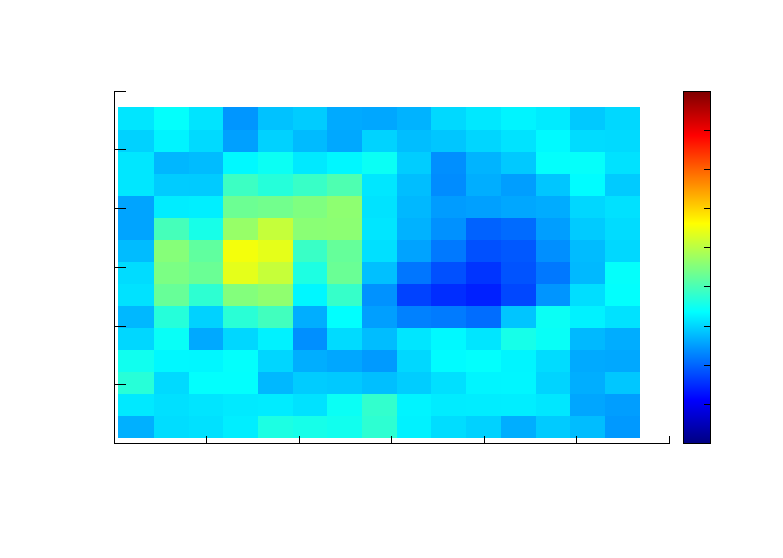
\includegraphics{plots/2DMRI200}}%
    \gplfronttext
  \end{picture}%
\endgroup

%         \caption{2D MRI mit T2 $\SI{200}{\milli\second}$}
%     \end{figure}
%     \begin{figure}[H]
%         \centering
%         \input{plots/2DMRI250.tex}
%         \caption{2D MRI mit T2 $\SI{250}{\milli\second}$}
%     \end{figure}
%     \begin{figure}[H]
%         \centering
%         \input{plots/2DMRI300.tex}
%         \caption{2D MRI mit T2 $\SI{300}{\milli\second}$}
%     \end{figure}
%     \begin{figure}[H]
%         \centering
%         \input{plots/2DMRI450.tex}
%         \caption{2D MRI mit T2 $\SI{450}{\milli\second}$}
%     \end{figure}
%     \begin{figure}[H]
%         \centering
%         \input{plots/2DMRI550.tex}
%         \caption{2D MRI mit T2 $\SI{550}{\milli\second}$}
%     \end{figure}

\begin{figure}[H]
    \centering
    \subfigure{\input{plots/2DMRI600.tex}}
    \subfigure{\input{plots/2DMRI1300.tex}}
    \subfigure{\input{plots/2DMRI2100.tex}}
    \subfigure{\input{plots/2DMRI2800.tex}}
    \caption{Links oben: 2DMRI mit T1 $\SI{600}{\milli\second}$;\\ Rechts oben: 2DMRI T1 $\SI{1300}{\milli\second}$;\\
    Links oben: 2DMRI T1 $\SI{2100}{\milli\second}$;\\ Rechts unten: 2DMRI T1 $\SI{2800}{\milli\second}$}
    \label{fig:Energieschema}
\end{figure}
\begin{figure}[H]
    \centering
    \subfigure{% GNUPLOT: LaTeX picture with Postscript
\begingroup
  % Encoding inside the plot.  In the header of your document, this encoding
  % should to defined, e.g., by using
  % \usepackage[cp1252,<other encodings>]{inputenc}
  \inputencoding{cp1252}%
  \makeatletter
  \providecommand\color[2][]{%
    \GenericError{(gnuplot) \space\space\space\@spaces}{%
      Package color not loaded in conjunction with
      terminal option `colourtext'%
    }{See the gnuplot documentation for explanation.%
    }{Either use 'blacktext' in gnuplot or load the package
      color.sty in LaTeX.}%
    \renewcommand\color[2][]{}%
  }%
  \providecommand\includegraphics[2][]{%
    \GenericError{(gnuplot) \space\space\space\@spaces}{%
      Package graphicx or graphics not loaded%
    }{See the gnuplot documentation for explanation.%
    }{The gnuplot epslatex terminal needs graphicx.sty or graphics.sty.}%
    \renewcommand\includegraphics[2][]{}%
  }%
  \providecommand\rotatebox[2]{#2}%
  \@ifundefined{ifGPcolor}{%
    \newif\ifGPcolor
    \GPcolorfalse
  }{}%
  \@ifundefined{ifGPblacktext}{%
    \newif\ifGPblacktext
    \GPblacktexttrue
  }{}%
  % define a \g@addto@macro without @ in the name:
  \let\gplgaddtomacro\g@addto@macro
  % define empty templates for all commands taking text:
  \gdef\gplbacktext{}%
  \gdef\gplfronttext{}%
  \makeatother
  \ifGPblacktext
    % no textcolor at all
    \def\colorrgb#1{}%
    \def\colorgray#1{}%
  \else
    % gray or color?
    \ifGPcolor
      \def\colorrgb#1{\color[rgb]{#1}}%
      \def\colorgray#1{\color[gray]{#1}}%
      \expandafter\def\csname LTw\endcsname{\color{white}}%
      \expandafter\def\csname LTb\endcsname{\color{black}}%
      \expandafter\def\csname LTa\endcsname{\color{black}}%
      \expandafter\def\csname LT0\endcsname{\color[rgb]{1,0,0}}%
      \expandafter\def\csname LT1\endcsname{\color[rgb]{0,1,0}}%
      \expandafter\def\csname LT2\endcsname{\color[rgb]{0,0,1}}%
      \expandafter\def\csname LT3\endcsname{\color[rgb]{1,0,1}}%
      \expandafter\def\csname LT4\endcsname{\color[rgb]{0,1,1}}%
      \expandafter\def\csname LT5\endcsname{\color[rgb]{1,1,0}}%
      \expandafter\def\csname LT6\endcsname{\color[rgb]{0,0,0}}%
      \expandafter\def\csname LT7\endcsname{\color[rgb]{1,0.3,0}}%
      \expandafter\def\csname LT8\endcsname{\color[rgb]{0.5,0.5,0.5}}%
    \else
      % gray
      \def\colorrgb#1{\color{black}}%
      \def\colorgray#1{\color[gray]{#1}}%
      \expandafter\def\csname LTw\endcsname{\color{white}}%
      \expandafter\def\csname LTb\endcsname{\color{black}}%
      \expandafter\def\csname LTa\endcsname{\color{black}}%
      \expandafter\def\csname LT0\endcsname{\color{black}}%
      \expandafter\def\csname LT1\endcsname{\color{black}}%
      \expandafter\def\csname LT2\endcsname{\color{black}}%
      \expandafter\def\csname LT3\endcsname{\color{black}}%
      \expandafter\def\csname LT4\endcsname{\color{black}}%
      \expandafter\def\csname LT5\endcsname{\color{black}}%
      \expandafter\def\csname LT6\endcsname{\color{black}}%
      \expandafter\def\csname LT7\endcsname{\color{black}}%
      \expandafter\def\csname LT8\endcsname{\color{black}}%
    \fi
  \fi
    \setlength{\unitlength}{0.0500bp}%
    \ifx\gptboxheight\undefined%
      \newlength{\gptboxheight}%
      \newlength{\gptboxwidth}%
      \newsavebox{\gptboxtext}%
    \fi%
    \setlength{\fboxrule}{0.5pt}%
    \setlength{\fboxsep}{1pt}%
\begin{picture}(7200.00,5040.00)%
    \gplgaddtomacro\gplbacktext{%
    }%
    \gplgaddtomacro\gplfronttext{%
      \csname LTb\endcsname%%
      \put(936,688){\makebox(0,0){\strut{}$0$}}%
      \put(1824,688){\makebox(0,0){\strut{}$20$}}%
      \put(2712,688){\makebox(0,0){\strut{}$40$}}%
      \put(3600,688){\makebox(0,0){\strut{}$60$}}%
      \put(4488,688){\makebox(0,0){\strut{}$80$}}%
      \put(5376,688){\makebox(0,0){\strut{}$100$}}%
      \put(6264,688){\makebox(0,0){\strut{}$120$}}%
      \put(3600,358){\makebox(0,0){\strut{}Y in $\si{\milli \meter}$}}%
      \put(700,938){\makebox(0,0)[r]{\strut{}$0$}}%
      \put(700,1502){\makebox(0,0)[r]{\strut{}$20$}}%
      \put(700,2066){\makebox(0,0)[r]{\strut{}$40$}}%
      \put(700,2630){\makebox(0,0)[r]{\strut{}$60$}}%
      \put(700,3194){\makebox(0,0)[r]{\strut{}$80$}}%
      \put(700,3758){\makebox(0,0)[r]{\strut{}$100$}}%
      \put(700,4322){\makebox(0,0)[r]{\strut{}$120$}}%
      \put(238,2630){\rotatebox{-270}{\makebox(0,0){\strut{}Z in $\si{\milli \meter}$}}}%
      \put(6795,938){\makebox(0,0)[l]{\strut{}$-3000$}}%
      \put(6795,1314){\makebox(0,0)[l]{\strut{}$-2000$}}%
      \put(6795,1690){\makebox(0,0)[l]{\strut{}$-1000$}}%
      \put(6795,2066){\makebox(0,0)[l]{\strut{}$0$}}%
      \put(6795,2442){\makebox(0,0)[l]{\strut{}$1000$}}%
      \put(6795,2818){\makebox(0,0)[l]{\strut{}$2000$}}%
      \put(6795,3194){\makebox(0,0)[l]{\strut{}$3000$}}%
      \put(6795,3570){\makebox(0,0)[l]{\strut{}$4000$}}%
      \put(6795,3946){\makebox(0,0)[l]{\strut{}$5000$}}%
      \put(6795,4322){\makebox(0,0)[l]{\strut{}$6000$}}%
    }%
    \gplbacktext
    \put(0,0){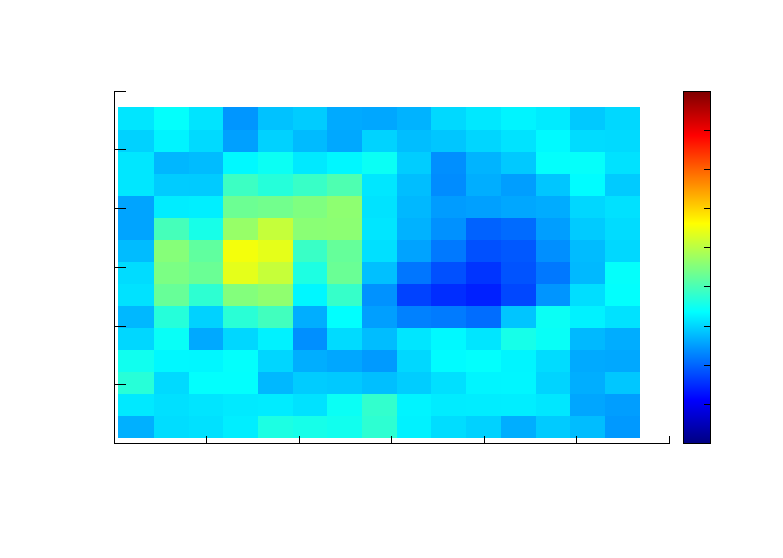
\includegraphics{plots/2DMRI200}}%
    \gplfronttext
  \end{picture}%
\endgroup
}
    \subfigure{\input{plots/2DMRI250.tex}}
    \subfigure{\input{plots/2DMRI450.tex}}
    \subfigure{\input{plots/2DMRI550.tex}}
    \caption{Links oben: 2DMRI T2 $\SI{200}{\milli\second}$;\\ Rechts oben: 2DMRI T2 $\SI{250}{\milli\second}$;\\
    Links oben: 2DMRI T2 $\SI{450}{\milli\second}$;\\ Rechts unten: 2DMRI T2 $\SI{550}{\milli\second}$}
    \label{fig:Energieschema}
\end{figure}
% !TEX root = main.tex
\subsection{J-Kopplung zur chemischen Strukturanalyse}
Eine weitere Anwendung der NMR-Technologie stellt die Möglichkeit dar chemische Strukturen zu analysieren.
Im vorliegenden Beispiel soll dabei Difluorobenzene untersucht werden.
Dabei wird die Verbindung zum einen auf die Kopplungskostante zwischen den einzelnen Fluor- und Wasserstoffatomen analysiert, dabei kann ermittelt werden, ob schwache Kopplung vorliegt zudem sollen auch Verhältnisse der Peakgrößen betrachtet werden.
Zunächst sollen daher einige grundlegende Zusammenhänge erläutert werden.
Da es sich bei dem vorliegenden Molekül um eine hetero-nukleare Verbindung zwischen Fluor (\ce{^19F}) und Wasserstoff (\ce{^1H}) handelt und der Versuchsaufbau während des Experiments auf die Larmorfrequenz von Wasserstoff ($\omega_{\text{L,H}} = \SI{1839}{\per \second}$) ausgerichtet ist müssen zunächst justierungen vorgenommen werden.
Dabei kann nach
\begin{align}
    \omega = \gamma \cdot B , \label{eq: LarmorB}    
\end{align}
die Larmorfrequenz für Fluor ($\omega_{\text{L,F}} = \SI{1730}{\per \second}$) berechnet werden. 
Die gyromagnetischen Verhältnisse $\gamma$ von Wasserstoff ($\gamma = \SI{2.675 e8}{\per \second \per \tesla}$) und Fluor ($\gamma = \SI{2.517 e8}{\per \second \per \tesla}$) wurden dabei \cite{Schmidt} entnommen. 
Das anliegende B-Feld war aus dem bis dato verwendeten Setups bekannt.
Anschließend wurde abermals nach Formel \eqref{eq: larmorcalc} die Kapazität des Schwingkreises ermittelt und ebenfalls auf die Larmorfrequenz abgestimmt.
Somit konnte ein Spektrum für Fluor angezeigt und die entsprechenden Parameter weiter optimiert werden. \cite{Schmidt} \\
Um anschließend beide Elemente gleichermaßen abbilden zu können, wurde sowohl der Mittelwert der Larmorfrequenzen ($\omega_{\text{L,MW}} = \SI{1787}{\per \second}$) wie auch der Kapazitäten ($C_{\text{MW}} = \SI{14.7}{\nano \farad}$) eingestellt und damit eine ,,Pulse and Collect''-Messung durchgeführt.

Dabei soll zunächst erläutert werden, welche Erkentnisse aus dem gewonnen Spektrum gewonnen werden können und welche Ergebnisse zu erwarten sind.


Abbildung \ref{fig:JKSchema} zeigt schematisch ein zu erwartendes Spektrum entnommen aus \cite{Schmidt}.
\begin{figure}[H]
    \centering
    \includegraphics[width= 0.75\textwidth]{Abbildungen/JKopplungSchema.png} 
    \caption[Schematische Darstellung eines Spektrums zur veranschaulichung der erwartbaren Ergebnisse durch die Analyse der J-Kopplung.]{Die Abbildung zeigt schematisch ein Spektrum für Trifluoroethanol.
    Dabei ist zu erkennen, welche Erkentnisse aus dem Spektrum abgelesen werden können.
    Diese sind zum einen die Kopplungskostante $J$, welche als Abstand zwischen den Peaks eines Elements verstanden wird, zum anderen kann die Annahme der schwachen Kopplung nach Formel \eqref{eq:SchwacheKopplung} überprüft werden.
    Zudem kann aus dem Verhältnis der Peakintegrale die Verteilung der Intensitäten berechnet werden.
    Diese folgt abhängig der Anzahl auftretender Maxima dem \textsc{Pascal}'schen Dreieck.}
    \label{fig:JKSchema}
\end{figure}

Hierbei ist allerdings ein anderes Molekül, Trifluoroethanol, veranschaulicht.
Erkennbar ist, dass aus dem Abstand der einzelnen Peakmaxima bei Fluor und Wasserstoff die Kopplungskonstante $J$ bestimmt werden kann.
Im Falle schwacher Kopplung gilt zudem die Relation
\begin{align}
    2 \pi \cdot J \ll \vert \omega_1 - \omega_2 \vert , \label{eq:SchwacheKopplung}
\end{align}
zwischen Kopplungskonstante $J$ und dem Abstand der Hauptmaxima $\vert \omega_1 - \omega_2 \vert$ der beiden Elemente.
Hierbei wird angenommen, dass bei der \textsc{Zeeman}-Wechselwirkung lediglich ein Störterm erster Ordnung durch die J-Kopplung berücksichtigt werden muss.
Sollten Störungen höherer Ordnung aufgrund stärkerer Kopplung vorliegen, so können diese die Peakbreite beeinflussen und vergrößern.
Zuletzt ist die Verteilung der Peakintensitäten, beziehungsweise das Verhältnis derer zueinander dargestellt.
Diese folgen je nach Anzahl der vorliegenden Peaks pro Element einer Verteilung nach dem \textsc{Pascal}'schen Dreieck.
Ermittelt wird diese Verteilung durch die Integration über die Peaks.
Die Anzahl vorliegender Peaks ist dadurch bestimmt wieviele Spins pro Element zur Wechselwirkung beitragen.
Hat ein Element $N$ Spins, so spaltet das andere Element in $N+1$ Peaks auf.
Entsprechend sind im vorliegenden Molekül je drei Maxima pro Element zu erwarten. 

Abbildung \ref{fig:JKopplungExp} zeigt das am Versuchstag gewonnene Spektrum.
Hierbei sind farbig (blau für Fluor und grün für Wasserstoff) die jeweils drei \textsc{Gauss}-Fits zu erkennen. 
Bei \SI{1750}{\hertz} ist zudem ein Peak zu erkennen, welcher wie bereits beschrieben auf die Taktung der deutschen Netzspannung zurückzuführen ist.

\begin{figure}[H]
    \centering
    \input{plots/JKopplung.tex}
    \caption{TODO!!;\\
    Zum tunen benutzte Daten des Puls and collect Experiments; Man soll noch die Integrale berechnen der einzelnen Peaks(aus den Integralen bekommt man dann das Verhältnuis von 1:2:3:3:2:1 oder so halt); Diese Peaks fitten bzw den abstand der Maximas berechnen=< daraus dann die Kopplungaskostante}
    \label{fig:JKopplungExp}
\end{figure}

Durch die \textsc{Gauss}-Fits konnten sowohl die Lage der Maxima, die Peakbreiten sowie die Integrale der Peaks berechnet werden.
Dabei wurde zudem die jeweilige Standardabweichung $\sigma$ als ein Fitparameter gewonnen, welche in Folge als Unsicherheit der Peakposition verwendet wurde.
Die Integrale der Peaks konnten dabei dadurch berechnet werden, dass das Integral über die \textsc{Gauss}'sche-Dichtefunktion
\begin{align}
    \frac{1}{\sqrt{2 \pi \sigma^2}} \exp{\left(-\frac{\left(x-\mu\right)^2}{2 \sigma^2}\right)}
\end{align}
auf $1$ normiert ist.
Diese wurde als Fitfunktion herangezogen.
Dabei beschreibt $\sigma$ die Standardabweichung, $\mu$ die Position des Maximums und ein weiterer Faktor $b$ kann daher den Wert des Integrals in guter Näherung angeben.

Somit ergaben sich für die Kopplungskonstanten folgende gewichtete Mittelwerte mit der jeweils zugehörigen kombinierten Unsicherheit, welche aus der jeweiligen Standardabweichung fortgeführt wurde:
\begin{align*}
    J_{\text{F}} = \SI{6.4 \pm 1.1}{\hertz} \\
    J_{\text{H}} = \SI{6.27 \pm 0.74}{\hertz} \\
    J_{\text{MW}} = \SI{6.3 \pm 1.3}{\hertz}
\end{align*}
Da diese ohnehin übereinstimmen sollten, bestätigen sich die berechneten Werte gegenseitig.
Zudem wurde eine Kopplungskonstante von $\SI{6}{\hertz}$ auf Grundlage der am Versuchstag vorliegenden Gegebenheiten erwartet.
Entsprechend bestätigen die Ergebnisse hier die Vorhersagen.
Die berechneten Unsicherheiten liegen zudem in einer sinnvollen Größenordnung und unterstreichen die Genauigkeit der Ergebnisse.

Bezüglich der Annahme der schwachen Kopplung konnte der Abstand der Hauptmaxima $\vert \omega_1 - \omega_2 \vert$ bestimmt werden und die Hypothese mittels Relation \eqref{eq:SchwacheKopplung} überprüft werden.
Hierbei ergab sich folgender Zusammenhang:
\begin{align*}
    2 \pi \cdot \SI{6.3}{\hertz} &\ll \vert \SI{1730}{\per \second} - \SI{1840}{\per \second} \vert \\
    <\approx > \quad \SI{6}{\hertz} &\ll \SI{18}{\hertz}
\end{align*}
Dabei genügt es ein Abschätzung vorzunehmen, weswegen keine exakten Werte berechnet wurden und auch auf die Angabe der Unsicherheiten verzichtet wurde.
Hierbei ist zu konstatieren, dass die Kopplungskonstante zwar kleiner, als der Abstand der Hauptmaxima ist, jedoch nicht signifikant.
Die Annahme der schwachen Kopplung kann folglich nicht bestätigt werden.
Daher ist mit einem Aufweiten der Peaks im Spektrum zu rechnen, was sich auch in den Werten der Peakintegrale widerspiegeln sollte.
\begin{table}[H]
    \centering
    \caption{Übersicht über die berechneten Peakintegrale der J-Kopplung.}
    \begin{tabular}{|l||r|r|r|} \hline
        Element & Peakposition in \si{\hertz} & rel. Peakintegral & Standardabweichung $\sigma$ \\ \hline \hline
        Fluor & \SI{1724.3 \pm 1.0}{} & \SI{1 \pm 0.63}{} & \SI{1.0}{}\\ \hline
        Fluor & \SI{1730.6 \pm 1.1}{}& \SI{1.54 \pm 0.54}{} & \SI{1.1}{}\\ \hline
        Fluor & \SI{1737.0 \pm 1.0}{} &\SI{1 \pm 0.41}{}& \SI{1.0}{}\\ \hline \hline
        Wasserstoff & \SI{1833.79 \pm 0.67}{} & \SI{1 \pm 0.55}{}& \SI{0.67}{}\\ \hline
        Wasserstoff & \SI{1840.11 \pm 0.81}{} & \SI{2.4 \pm 0.77}{}& \SI{0.81}{}\\ \hline
        Wasserstoff & \SI{1846.34 \pm 0.65}{}  & \SI{0.84 \pm 0.39}{}& \SI{0.65}{}\\ \hline
    \end{tabular} 
    \label{tab:Peaksintens} 
\end{table}
Tabelle \ref{tab:Peaksintens} zeigt eine Übersicht über die relativen Peakintegrale.
Dabei wurden die relativen Integrale jeweils auf den Wert des Maximums welches bei der geringsten Frequenz auftrat normiert.
Die angegebenen Unsicherheiten wurden dabei \textit{GnuPlot} entnommen und nach der Formel zur kombinierten Unsicherheit fortgeführt.
Hierbei zeigt sich, dass zwar teilweise ein Verteilung nach dem \textsc{Pascal}'schen Dreieck (1:2:1) unter Berücksichtigung der berechneten Unsicherheiten vorliegt, diese jedoch im Verhältnis zu den berechneten relativen Peakintegralen recht groß ausfallen.
Die absoluten Werte lassen somit ebenfalls darauf schließen, dass die Annahme der schwachen Kopplung nicht erfüllt sein könnte und somit die Peaks aufgeweitet auftreten.
Unterstrichen wird dies durch die Betrachtung der Standardabweichung der Peaks in Tabelle \ref{tab:Peaksintens}. 
Insbesondere bei Wasserstoff liegt offenbar ein Unterschied bei der Standardabweichung zwischen dem Haupt- und den Nebenmaxima vor.
Dieser Unterschied in der Peakweite, welcher durch $\sigma$ charakterisiert wird belegt das Aufweiten der Peaks.
Zudem wurde während der Versuchsdurchführung versucht ein möglichst rauschfreies Spektrum mit recht eindeutigen Maxima zu erhalten.
Um dies zu gewährleisten wurde die Anzahl der aufgenommenen Datenpunkte reduziert.
Dies führt dazu, dass pro Fit nur wenige Datenpunkte erfasst werden konnten.
Dadurch liegt der Schluss nahe, dass zum einen die angegebenen Unsicherheiten womöglich zu klein sind und zum anderen hätten mehr Datenpunkte zu verlässlicheren Ergebnissen geführt.
Die Abweichungen in den Peakintegralen könnten folglich auch von diesem Umstand beeinflusst sein.
Insgesamt kann also festgehalten werden, dass vor allem bei der Betrachtung der Kopplungskonstante gute Übereinstimmungen mit der Theorie beziehungsweise den Erwartungen erzielt wurden.
Zudem ließen die Betrachtung der schwachen Wechselwirkung und der Peakintegrale interessante Rückschlüsse zu und förderten eine kritische Auseinandersetzung mit selbigen, auch wenn die quantitativen Betrachtung durchaus den Schluss zulassen, dass Optimierungen am Versucshaufbau und während der Durchführung denkbar sind.




% !TEX root = main.tex
\section{T1 und T2 Relaxationszeit für Wasser und mit Zusatzmitteln}
\begin{figure}[H]
    \centering
    % !TEX root = main.tex
\section{T1 und T2 Relaxationszeit für Wasser und mit Zusatzmitteln}
\begin{figure}[H]
    \centering
    \input{plots/T2Wasser.tex}
    \caption{T2 Messung von Wasser}
\end{figure}
    \caption{Diffusionskoeffizient $\SI{3e-9}{\frac{\m^2}{s}}$}
\end{figure}
%----------------------------------------------------------------%
%----------------------Fazit-------------------------------------%
%----------------------------------------------------------------%
\newpage
% !TEX root = main.tex
\section{Fehlerdiskussion und Fazit}
% \label{sec:Fazit}
\newpage
%----------------------------------------------------------------%
%----------------------Verzeichnisse-----------------------------%
%----------------------------------------------------------------%
% !TEX root = main.tex
\bibliography{literatur}
\bibliographystyle{babalpha}
\newpage
\listoffigures
\listoftables
\addcontentsline{toc}{section}{Attachments}
\section*{Attachments}
\setcounter{section}{6}
\newpage


\begin{table}[H]
    \centering
    \caption{$T_1$ und $T_2$ abhängig vom Kontrastmittel und dessen Konzentration.}
    \begin{tabular}{lllll}  \hline
    \multicolumn{1}{|l||}{}            & \multicolumn{1}{l|}{T1 in \si{\milli \second}}      & \multicolumn{1}{l|}{U(T1)-Fit in \si{\milli \second}} & \multicolumn{1}{l|}{T2 in \si{\milli \second}}      & \multicolumn{1}{l|}{U(T2)-Fit in \si{\milli \second}}  \\ \hline
    \multicolumn{1}{|l||}{Wasser}      & \multicolumn{1}{l|}{2199,46} & \multicolumn{1}{l|}{0,003027}  & \multicolumn{1}{l|}{1901,06} & \multicolumn{1}{l|}{89,83}      \\ \hline \hline
    \multicolumn{1}{|l||}{\ce{Cu^2+}    ($\SI{0.5}{\frac{\mol}{\metre \tothe{3}}}$)}  & \multicolumn{1}{l|}{1394,84} & \multicolumn{1}{l|}{0,001055}  & \multicolumn{1}{l|}{1215,51} & \multicolumn{1}{l|}{0,0002529}  \\ \hline
    \multicolumn{1}{|l||}{\ce{Cu^2+}    ($\SI{1.0}{\frac{\mol}{\metre \tothe{3}}}$)}  & \multicolumn{1}{l|}{1003,4}  & \multicolumn{1}{l|}{0,0004851} & \multicolumn{1}{l|}{1066,44} & \multicolumn{1}{l|}{0,0002621}  \\ \hline
    \multicolumn{1}{|l||}{\ce{Cu^2+}    ($\SI{2.0}{\frac{\mol}{\metre \tothe{3}}}$)} & \multicolumn{1}{l|}{646,849} & \multicolumn{1}{l|}{71,54}     & \multicolumn{1}{l|}{748,404} & \multicolumn{1}{l|}{0,0001937}  \\ \hline
    \multicolumn{1}{|l||}{\ce{Cu^2+}    ($\SI{4.0}{\frac{\mol}{\metre \tothe{3}}}$)} & \multicolumn{1}{l|}{431,268} & \multicolumn{1}{l|}{0,0002906} & \multicolumn{1}{l|}{341,83}  & \multicolumn{1}{l|}{0,0001228}  \\ \hline \hline
    \multicolumn{1}{|l||}{\ce{Mn^2+}    ($\SI{0.05}{\frac{\mol}{\metre \tothe{3}}}$)}     & \multicolumn{1}{l|}{1178,28} & \multicolumn{1}{l|}{0,0009801} & \multicolumn{1}{l|}{548,337} & \multicolumn{1}{l|}{0,0001258}  \\ \hline
    \multicolumn{1}{|l||}{\ce{Mn^2+}    ($\SI{0.10}{\frac{\mol}{\metre \tothe{3}}}$)}     & \multicolumn{1}{l|}{725,857} & \multicolumn{1}{l|}{0,0006027} & \multicolumn{1}{l|}{279,858} & \multicolumn{1}{l|}{0,00008179} \\ \hline
    \multicolumn{1}{|l||}{\ce{Mn^2+}    ($\SI{0.20}{\frac{\mol}{\metre \tothe{3}}}$)}    & \multicolumn{1}{l|}{316,085} & \multicolumn{1}{l|}{0,0003079} & \multicolumn{1}{l|}{170,996} & \multicolumn{1}{l|}{0,0001182}  \\ \hline
    \multicolumn{1}{|l||}{\ce{Mn^2+}    ($\SI{0.40}{\frac{\mol}{\metre \tothe{3}}}$)}    & \multicolumn{1}{l|}{180,244} & \multicolumn{1}{l|}{0,0001274} & \multicolumn{1}{l|}{69,1512} & \multicolumn{1}{l|}{0,0000547}  \\ \hline
    \end{tabular}
    \label{tab:T1T2Kontrast}
\end{table}

\begin{figure}[H]
    \centering
    \input{plots/Relaxivitat_CuT2.tex}
    \caption{Bestimmung der Relaxivität $r_2$ mit Kupfer als Kontrastmittel. Analog zu Abbildung \ref{fig:RelaxCUT1}.}
    \label{fig:RelaxCUT2}
\end{figure}

\begin{figure}[H]
    \centering
    \input{plots/Relaxivitat_MnT1.tex}
    \caption{Bestimmung der Relaxivität $r_1$ mit Mangna als Kontrastmittel. Analog zu Abbildung \ref{fig:RelaxCUT1}.}
    \label{fig:RelaxMNT1}
\end{figure}

\begin{figure}[H]
    \centering
    % GNUPLOT: LaTeX picture with Postscript
\begingroup
  % Encoding inside the plot.  In the header of your document, this encoding
  % should to defined, e.g., by using
  % \usepackage[cp1252,<other encodings>]{inputenc}
  \inputencoding{cp1252}%
  \makeatletter
  \providecommand\color[2][]{%
    \GenericError{(gnuplot) \space\space\space\@spaces}{%
      Package color not loaded in conjunction with
      terminal option `colourtext'%
    }{See the gnuplot documentation for explanation.%
    }{Either use 'blacktext' in gnuplot or load the package
      color.sty in LaTeX.}%
    \renewcommand\color[2][]{}%
  }%
  \providecommand\includegraphics[2][]{%
    \GenericError{(gnuplot) \space\space\space\@spaces}{%
      Package graphicx or graphics not loaded%
    }{See the gnuplot documentation for explanation.%
    }{The gnuplot epslatex terminal needs graphicx.sty or graphics.sty.}%
    \renewcommand\includegraphics[2][]{}%
  }%
  \providecommand\rotatebox[2]{#2}%
  \@ifundefined{ifGPcolor}{%
    \newif\ifGPcolor
    \GPcolorfalse
  }{}%
  \@ifundefined{ifGPblacktext}{%
    \newif\ifGPblacktext
    \GPblacktexttrue
  }{}%
  % define a \g@addto@macro without @ in the name:
  \let\gplgaddtomacro\g@addto@macro
  % define empty templates for all commands taking text:
  \gdef\gplbacktext{}%
  \gdef\gplfronttext{}%
  \makeatother
  \ifGPblacktext
    % no textcolor at all
    \def\colorrgb#1{}%
    \def\colorgray#1{}%
  \else
    % gray or color?
    \ifGPcolor
      \def\colorrgb#1{\color[rgb]{#1}}%
      \def\colorgray#1{\color[gray]{#1}}%
      \expandafter\def\csname LTw\endcsname{\color{white}}%
      \expandafter\def\csname LTb\endcsname{\color{black}}%
      \expandafter\def\csname LTa\endcsname{\color{black}}%
      \expandafter\def\csname LT0\endcsname{\color[rgb]{1,0,0}}%
      \expandafter\def\csname LT1\endcsname{\color[rgb]{0,1,0}}%
      \expandafter\def\csname LT2\endcsname{\color[rgb]{0,0,1}}%
      \expandafter\def\csname LT3\endcsname{\color[rgb]{1,0,1}}%
      \expandafter\def\csname LT4\endcsname{\color[rgb]{0,1,1}}%
      \expandafter\def\csname LT5\endcsname{\color[rgb]{1,1,0}}%
      \expandafter\def\csname LT6\endcsname{\color[rgb]{0,0,0}}%
      \expandafter\def\csname LT7\endcsname{\color[rgb]{1,0.3,0}}%
      \expandafter\def\csname LT8\endcsname{\color[rgb]{0.5,0.5,0.5}}%
    \else
      % gray
      \def\colorrgb#1{\color{black}}%
      \def\colorgray#1{\color[gray]{#1}}%
      \expandafter\def\csname LTw\endcsname{\color{white}}%
      \expandafter\def\csname LTb\endcsname{\color{black}}%
      \expandafter\def\csname LTa\endcsname{\color{black}}%
      \expandafter\def\csname LT0\endcsname{\color{black}}%
      \expandafter\def\csname LT1\endcsname{\color{black}}%
      \expandafter\def\csname LT2\endcsname{\color{black}}%
      \expandafter\def\csname LT3\endcsname{\color{black}}%
      \expandafter\def\csname LT4\endcsname{\color{black}}%
      \expandafter\def\csname LT5\endcsname{\color{black}}%
      \expandafter\def\csname LT6\endcsname{\color{black}}%
      \expandafter\def\csname LT7\endcsname{\color{black}}%
      \expandafter\def\csname LT8\endcsname{\color{black}}%
    \fi
  \fi
    \setlength{\unitlength}{0.0500bp}%
    \ifx\gptboxheight\undefined%
      \newlength{\gptboxheight}%
      \newlength{\gptboxwidth}%
      \newsavebox{\gptboxtext}%
    \fi%
    \setlength{\fboxrule}{0.5pt}%
    \setlength{\fboxsep}{1pt}%
\begin{picture}(7200.00,5040.00)%
    \gplgaddtomacro\gplbacktext{%
      \csname LTb\endcsname%%
      \put(682,704){\makebox(0,0)[r]{\strut{}$0$}}%
      \put(682,1733){\makebox(0,0)[r]{\strut{}$5$}}%
      \put(682,2762){\makebox(0,0)[r]{\strut{}$10$}}%
      \put(682,3790){\makebox(0,0)[r]{\strut{}$15$}}%
      \put(682,4819){\makebox(0,0)[r]{\strut{}$20$}}%
      \put(814,484){\makebox(0,0){\strut{}$0$}}%
      \put(2012,484){\makebox(0,0){\strut{}$0.1$}}%
      \put(3210,484){\makebox(0,0){\strut{}$0.2$}}%
      \put(4407,484){\makebox(0,0){\strut{}$0.3$}}%
      \put(5605,484){\makebox(0,0){\strut{}$0.4$}}%
      \put(6803,484){\makebox(0,0){\strut{}$0.5$}}%
    }%
    \gplgaddtomacro\gplfronttext{%
      \csname LTb\endcsname%%
      \put(308,2761){\rotatebox{-270}{\makebox(0,0){\strut{}Kehrwert der Zeit in $\si{\frac{1}{\second}}$}}}%
      \put(3808,154){\makebox(0,0){\strut{}Konzentration in  $\si{\frac{\mol}{\meter \tothe{3}}}$}}%
      \csname LTb\endcsname%%
      \put(5858,4606){\makebox(0,0)[r]{\strut{}$1/T_{\text{2}}\left([\ce{Mn^2+}]\right)$}}%
      \csname LTb\endcsname%%
      \put(5858,4386){\makebox(0,0)[r]{\strut{}linearer Fit}}%
    }%
    \gplbacktext
    \put(0,0){\includegraphics{plots/Relaxivitat_MnT2}}%
    \gplfronttext
  \end{picture}%
\endgroup

    \caption{Bestimmung der Relaxivität $r_2$ mit Mangan als Kontrastmittel. Analog zu Abbildung \ref{fig:RelaxCUT1}.}
    \label{fig:RelaxMNT2}
\end{figure}

\end{document}